\documentclass[%
specialist,  % тип документа
%natbib,      % использовать пакет natbib для "сжатия" цитирований
subf,        % использовать пакет subcaption для вложенной нумерации рисунков
href,        % использовать пакет hyperref для создания гиперссылок
colorlinks,  % цветные гиперссылки
%fixint,     % включить прямые знаки интегралов
]{disser}

\usepackage[
  a4paper, mag=1000,
  left=2.5cm, right=1cm, top=2cm, bottom=2cm, headsep=0.7cm, footskip=1cm
]{geometry}

\usepackage{ esint }
\usepackage[intlimits]{amsmath}
\usepackage{amssymb,amsfonts}
\usepackage{graphicx}
\usepackage[T2A]{fontenc}
\usepackage[utf8]{inputenc}
\usepackage[english,russian]{babel}
\ifpdf\usepackage{epstopdf}\fi
\usepackage[autostyle]{csquotes}

\usepackage{listings}
\usepackage{xcolor}
\definecolor{codegreen}{rgb}{0,0.6,0}
\definecolor{codegray}{rgb}{0.5,0.5,0.5}
\definecolor{codepurple}{rgb}{0.58,0,0.82}
\definecolor{backcolour}{rgb}{0.95,0.95,0.92}
\definecolor{codeorange}{rgb}{2.55,1.65,0.5}

\lstdefinestyle{mystyle}{
	backgroundcolor=\color{backcolour},   
	commentstyle=\color{codegreen},
	keywordstyle=\color{magenta},
	numberstyle=\tiny\color{codegray},
	stringstyle=\color{codepurple},
	basicstyle=\ttfamily\footnotesize,
	breakatwhitespace=false,         
	breaklines=true,                 
	captionpos=b,                    
	keepspaces=true,                 
	numbers=left,                    
	numbersep=5pt,                  
	showspaces=false,                
	showstringspaces=false,
	showtabs=false,                  
	tabsize=2
}

\lstset{style=mystyle}

% Шрифт Times в тексте как основной
%\usepackage{tempora}
% альтернативный пакет из дистрибутива TeX Live
%\usepackage{cyrtimes}

% Шрифт Times в формулах как основной
%\usepackage[varg,cmbraces,cmintegrals]{newtxmath}
% альтернативный пакет
%\usepackage[subscriptcorrection,nofontinfo]{mtpro2}

% Плавающие рисунки "в оборку".
\usepackage{wrapfig}

%\usepackage[style=gost-numeric,
%  backend=biber,
%  language=auto,
%  hyperref=auto,
%  autolang=other,
%  sorting=none
%]{biblatex}

%\addbibresource{thesis.bib}

%\renewcommand{\chaptername}{}
%\renewcommand{\bibname}{Литература}
%\renewcommand{\figurename}{Рисунок}

\graphicspath{{fig/}}
\renewcommand{\thechapterfont}{\normalsize\bfseries} % Номер главы полужирным
\renewcommand{\prethechapter}{} % Убираем слово "глава"
%\renewcommand{\postthechapter}{.~} % ставим точку и пробел после номер
%\renewcommand{\appendixfont}{\normalsize\bfseries}
%\renewcommand{\chapterfont}{\normalsize\bfseries}
%\renewcommand{\sectionfont}{\normalsize\bfseries}
%\renewcommand{\subsectionfont}{\normalsize\bfseries}
%\renewcommand{\subsubsectionfont}{\normalsize\bfseries}
%\renewcommand{\tocprethechapter}{} % в оглавлении убираем слово "Глава"
\renewcommand{\theappendixalign}{\hfill} % выключка вправо для слова "приложение" в приложениии
\renewcommand{\theappendix}{\arabic{chapter}} % заменяем нумерацию приложений на цифры
%\renewcommand{\pretheappendix}{\protect{ПРИЛОЖЕНИЕ}~} % Меняем регистр слова "Приложение"
%\renewcommand{\tocpretheappendix}{\protect{ПРИЛОЖЕНИЕ}~} % Меняем регистр слова "Приложение"
\renewcommand{\introname}{ВВЕДЕНИЕ}
%\renewcommand{\sectionindent}{1cm}
%\renewcommand{\subsectionindent}{1cm}
%\renewcommand{\aftersection}{6pt plus .1pt}
%\renewcommand{\aftersubsection}{3pt plus .1pt}
\renewcommand{\conclusionname}{ЗАКЛЮЧЕНИЕ}
%\renewcommand{\bibintoc}{Литература}

% Номера страниц снизу и по центру
%\pagestyle{footcenter}
%\chapterpagestyle{footcenter}

% Точка с запятой в качестве разделителя между номерами цитирований
%\setcitestyle{semicolon}

% Использовать полужирное начертание для векторов
\let\vec=\mathbf

% Включать подсекции в оглавление
\setcounter{tocdepth}{2}

\graphicspath{{fig/}}

\begin{document}

% Переопределение стандартных заголовков
\def\contentsname{Содержание}
%\def\conclusionname{Выводы}
%\def\bibname{Литература}

%
% Титульный лист на русском языке
%

% Название организации
\institution{~\\ МИНИСТЕРСТВО ОБРАЗОВАНИЯ И НАУКИ РОССИЙСКОЙ ФЕДЕРАЦИИ\\ «Нижегородский государственный университет
	им. Н.\,И.\,Лобачевского» \\
	Радиофизический факультет \\
	Кафедра электродинамики \\ 
	Направление «Радиофизика»}
% Имя лица, допускающего к защите (зав. кафедрой)


% Имя лица, допускающего к защите (зав. кафедрой)
%\apname{ФИО зав. кафедрой}

\title{ВЫПУСКНАЯ  КВАЛИФИКАЦИОННАЯ  РАБОТА}

\topic{ИССЛЕДОВАНИЕ ОСОБЕННОСТЕЙ РАССЕЯНИЯ ЭЛЕКТРОМАГНИТНЫХ ВОЛН НА ФРАКТАЛЬНЫХ ОБЪЕКТАХ}

% Автор
%\author{ФИО автора}
% Группа
%\group{Студента группы}

% Научный руководитель
\sa      {ФИО руководителя}
\sastatus{д.~ф.-м.~н., ст.~н.~с.}

% Рецензент
\rev      {П.\,П.~Петров}
\revstatus{к.\,ф.-м.\,н., доцент}

% Город и год
\city{Нижний Новгород}
\date{\number\year}

\maketitle

%%
%% Titlepage in English
%%
%
%\setlength\thirdskip{0pt}
%
%\institution{Name of Organization}
%
%% Approved by
%\apname{Professor S.\,S.~Sidorov}
%
%\title{Diploma Thesis}
%
%% Topic
%\topic{Dummy Title}
%
%% Author
%\author{Author's Name} % Full Name
%\group{} % Study Group
%
%% Scientific Advisor
%\sa       {I.\,I.~Ivanov}
%\sastatus {Professor}
%
%% Reviewer
%\rev      {P.\,P.~Petrov}
%\revstatus{Associate Professor}
%
%% Consultant
%\con{}
%\conspec{}
%\constatus{}
%
%% City & Year
%\city{Saint Petersburg}
%\date{\number\year}
%
%\maketitle[en]

% Содержание
\tableofcontents

% Введение
\intro

\clearpage

% Глава 1
\section{Постановка задачи и основные соотношения}
Будем рассматривать рассеяние плоской электромагнитной волны на рассеивателях в различных диапазонах частот для шариков, состоящих из серебра, меди и золота. Представим шарики ввиде сфер и рассмотрим три случая, для одиночной сферы Рис.\ref{fig:1st_scatterer}, для 5 сфер Рис.\ref{fig:2nd_scatterer} и для 17 сфер Рис.\ref{fig:3td_scatterer}. Однако пред этим, найдем рассеянние на цилиндре численным и точным методом решения, чтобы убедиться в правильности получаемых данных. \\
\begin{figure}[h!]
	\centering
	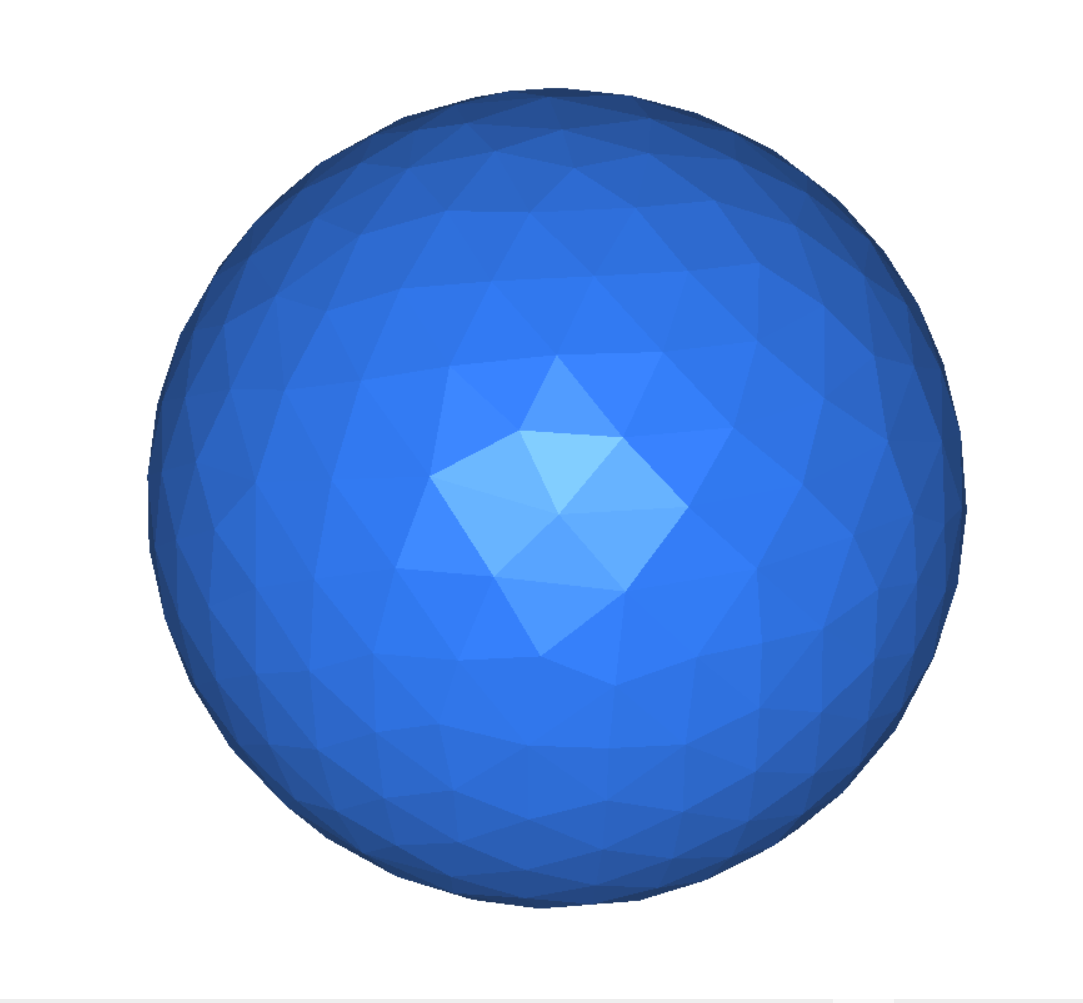
\includegraphics[width=0.4\linewidth]{1st_scatterer}
	\caption{Единичная сфера}
	\label{fig:1st_scatterer}
\end{figure} \\
\begin{figure}[h!]
	\centering
	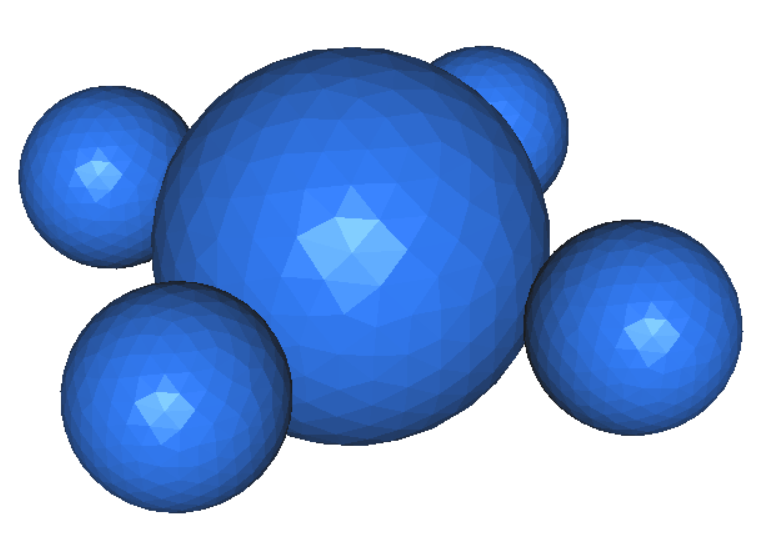
\includegraphics[width=0.5\linewidth]{2nd_scatterer}
	\caption{Первая итерация - 5 сфер}
	\label{fig:2nd_scatterer}
\end{figure} \\
\begin{figure}[h!]
	\centering
	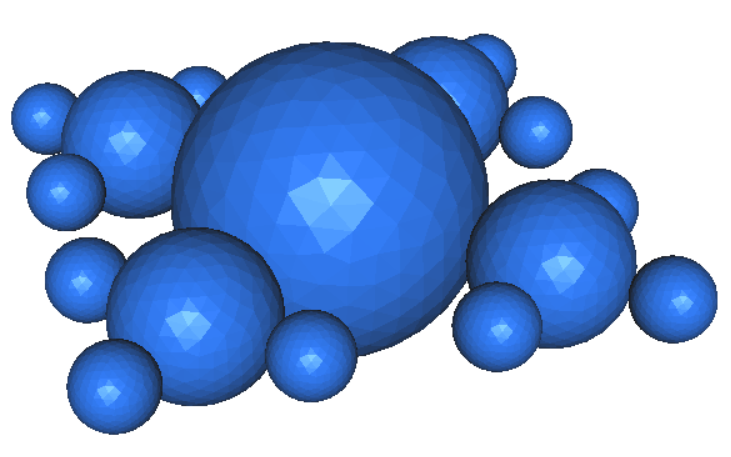
\includegraphics[width=0.5\linewidth]{3td_scatterer}
	\caption{Вторая итерация - 17 сфер}
	\label{fig:3td_scatterer}
\end{figure} \\
После этого решим задачу дифракции одиночной сферы используя метод конечных элементов. Для этого наш объект заключим в сферическую область, в которой будут рассеиваться волны. Сразу определим, что внутри нашего объекта область заполнена диэлектриком, а его радиус будет в 10 раз меньше длины волны принимаемой для расчетов ($ \lambda = 1 $), а радиус сферической области в 4 раза больше (Рис.\ref{fig:ces1}). Так же стоит отметить, что на протяжении всей работы будет использоваться гармоническая зависимость $ e^{j \omega t} $, где $ j = \sqrt{-1} $. Далее найдем сечение рассеяния $ \sigma_s $ и сечение поглощения $ \sigma_a $, которое будет находиться на удалении $ \lambda = 3 $, с помощью действительной $ \varepsilon' $ и мнимой $ \varepsilon'' $ части диэлектрической проницаемости на основе коэффициентов преломления $ n' $ и $ n'' $. Сделаем тоже самое для всех трех случаев.  Для удобства поиска решения расчеты будем производить в декартовой системе координат. \\
\begin{figure}[h!]
	\centering
	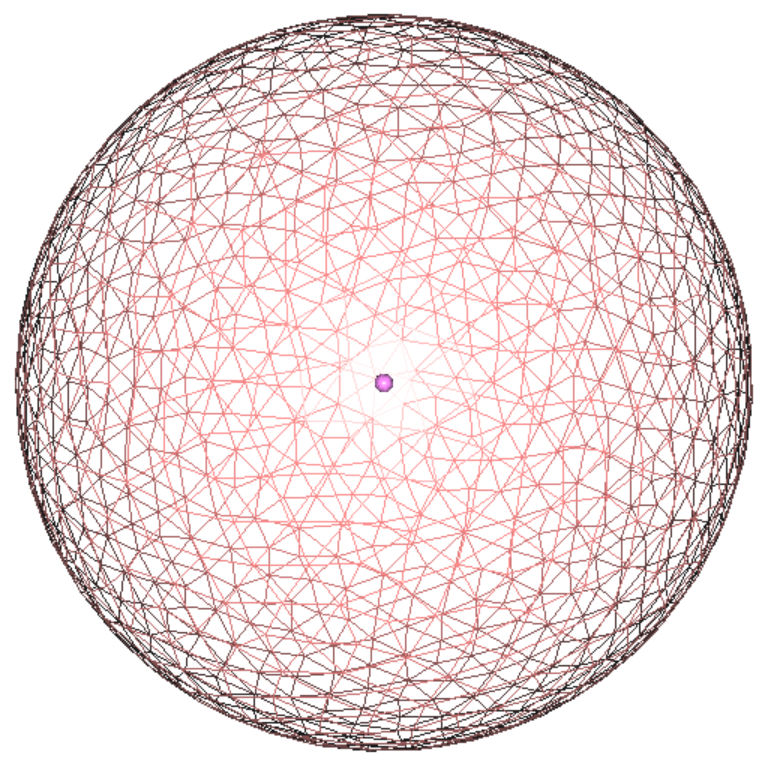
\includegraphics[width=0.4\linewidth]{ces1}
	\caption{}
	\label{fig:ces1}
\end{figure} \\
\newpage
На Рис.~\ref{fig:3td_scattererAndOuterSpheres} можно увидеть случай с 17 сферами, где в центре находится сам объект, окруженный сечением рассеяния, заключенный в сферическую область.\\
\begin{figure}[h!]
	\centering
	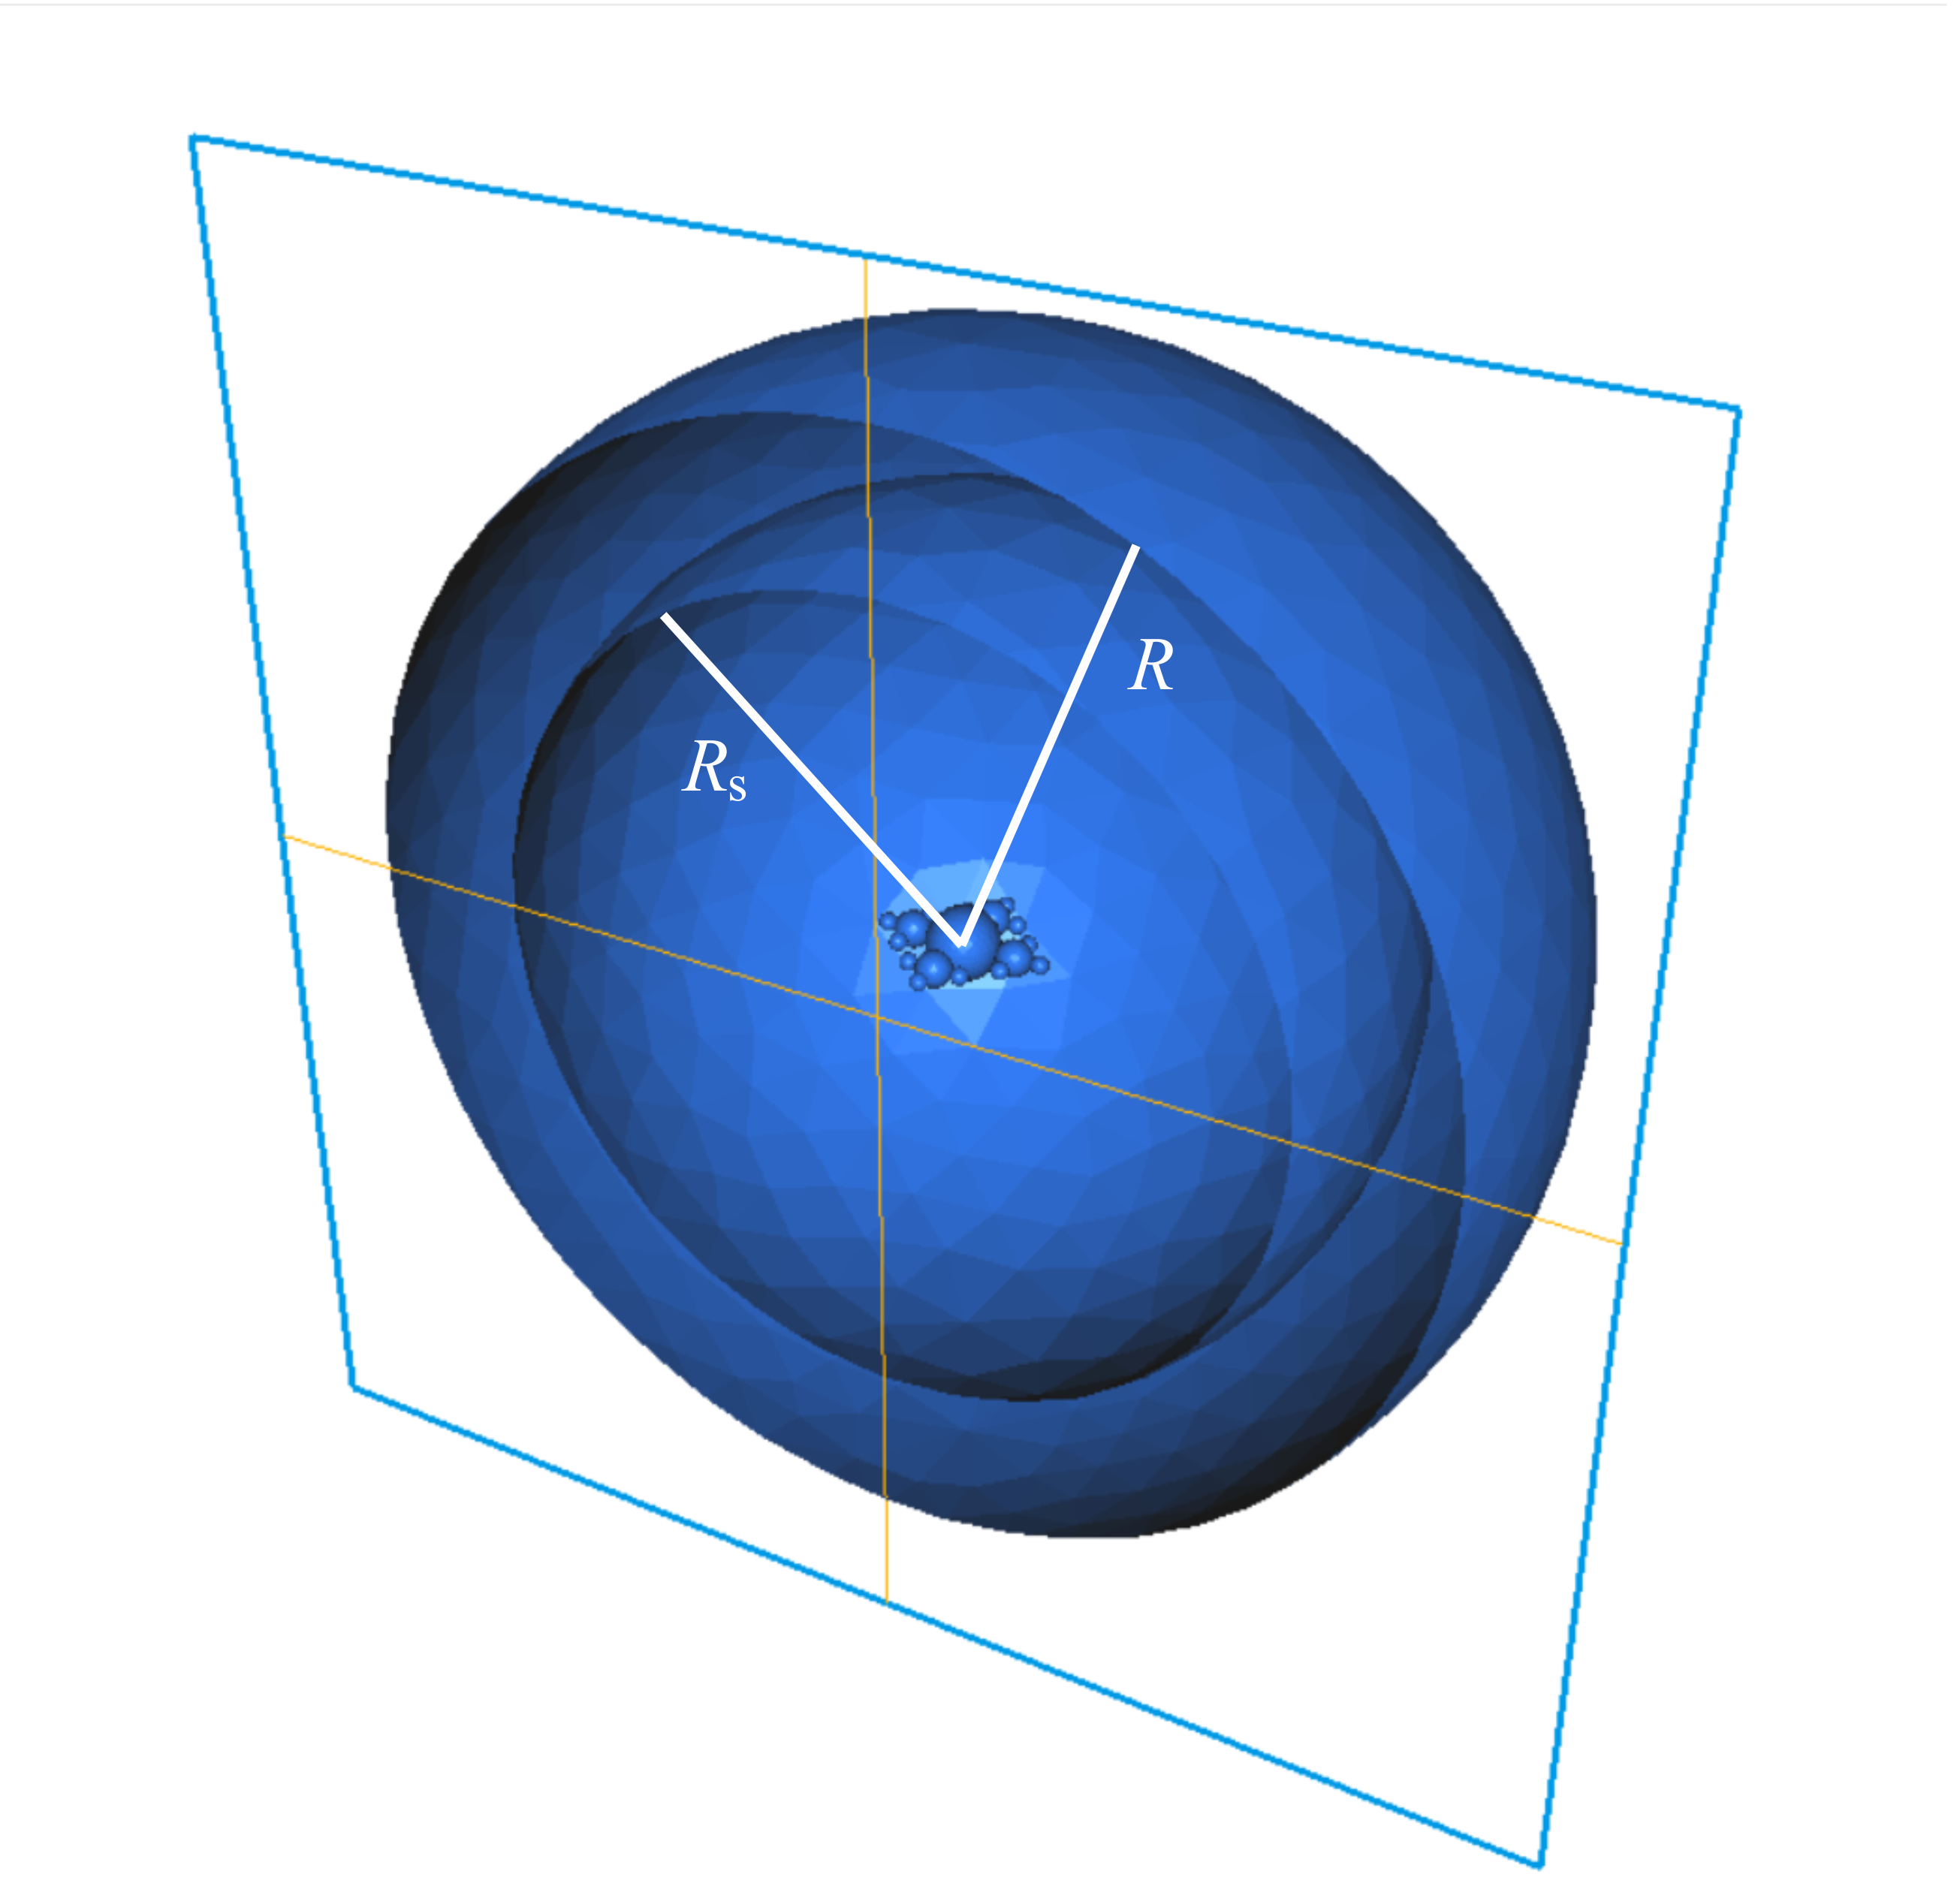
\includegraphics[width=0.6\linewidth]{3td_scattererAndOuterSpheres}
	\caption{}
	\label{fig:3td_scattererAndOuterSpheres}
\end{figure} \\
\section{Описание метода решения задачи}
Рассчеты для цилиндра будем производить в простейшем двумерном случае.
\\
В начале запишем уравнение Максвелла: \\
\begin{center}
	$ 	\rm rot\vec{E} = -\dfrac{1}{c}\dfrac{\partial \vec{B}}{\partial t} $ 
\end{center}
\begin{center}
	$ 	\rm rot\vec{H} =\dfrac{4\pi}{c}\vec{j} + \dfrac{1}{c}\dfrac{\partial \vec{D}}{\partial t} $
\end{center}
\begin{center}
	$ 	div\vec{D} = 4\pi \rho $
\end{center}
	\begin{center}
		$ div \vec{B} = 0 $, где
	\end{center} 
\begin{center}
	$ \vec{H} = \vec{r}_{0}H_{0}\rm cos(\omega t - kz) $, и $ \varepsilon = 1 $ \\
\end{center}
При этом не забыв про материальные уравнения, которые описывают характеристики среды, в которой распространяется электромагнитная волна,а именно наличие диэлектриков ($ \varepsilon $), ферромагнетиков ($ \mu $), удельной проводимости ($ \gamma $):
\begin{center}
	$ \vec{D} = \varepsilon_{0} \varepsilon \vec{E} $
\end{center}
\begin{center}
	$ \vec{B} = \mu_{0} \mu \vec{H} $
\end{center}
\begin{center}
	$ \vec{j} = \gamma \vec{E} $
\end{center}
Где $ \varepsilon_{0} $ и $ \mu_{0} $ - соответственно электрическая и магнитная постоянные, $ \varepsilon $ и $ \mu $ - диэлектрическая и магнитная проницаемости, $ \gamma $ - удельная проводимость вещества. \\
А так же запишем уравнение Гельмгольца:
\begin{center}
	$ \Delta H_{z} + k^2H_{z} = 0 $ 
\end{center}\\
Из этого получаем : \begin{center}
	$ \rm rot\vec{H} = ik_{0}\vec{H} $
\end{center}
Отсюда выражаем  \vec{E}: \\
\begin{center}
	$\vec{E} = - \dfrac{i}{k_{0}} \rm rot\vec{H} = - \dfrac{i}{k_{0}}(\vec{x_{0}}\dfrac{\partial \vec{H_{z}}}{\partial y} - \vec{y_{0}}\dfrac{\partial \vec{H_{z}}}{\partial x}) 
	$
\end{center}\\
А так же для $ E_{x} и E_{y} $ соответственно: \\
\begin{center}
	$ E_{x} = - 
	\dfrac{i}{k_{0}}
	\dfrac{\partial\vec{H_{z}}}{\partial y} \\
	E_{y} = \dfrac{i}{k_{0}}
	\dfrac{\partial\vec{H_{z}}}{\partial x} \\ $
\end{center} \\
Для условной поверхности S : \\
\begin{center}
	$ [\vec{n}, \vec{x_{0}}E_{x} + \vec{y_{0}}E_{y}] = 0 $
\end{center}\\
Таким образом получим интеграл:
\\
\begin{center}
	$ \int\limits_{V}^{} \Delta H_{z} \cdot wdv = - \int\limits_{V}^{}(\nabla H_{z}, \nabla w)dv +  \int\limits_{V}^{}(\nabla H_{z} \cdot w)dv
	$ \\
\end{center}
Так как один из интегралов правой части: 
\begin{center}
	$  \int\limits_{V}^{}(\nabla H_{z} \cdot w)dv $
\end{center} \\
Соответственно равен: 
\\
\begin{center}
	$\int\limits_{V}^{}(\nabla H_{z} \cdot w)dv = \oint\limits_{S}^{} \nabla H_{z}  wds \cdot \vec{n} = 0 $ \\
\end{center}
\\
То граничные условия в нашей задаче задавать нет необходимости.
Поэтому получим: \\
\begin{center}
	$ \nabla H_{z} = \vec{x}_{0} \dfrac{\partial\vec{H_{z}}}{\partial x} - \vec{y}_{0}
	\dfrac{\partial\vec{H_{z}}}{\partial y} $
	\\
\end{center}
Cоответственно используя нормали $n_{x}$ и $n_{y}$  запишем искомое уравнение:
\\
\begin{center}
	$ \vec{n}\nabla H_{z} = \dfrac{\partial\vec{H_{z}}}{\partial n} = 
	n_{x}\dfrac{\partial\vec{H_{z}}}{\partial x} +
	n_{y}\dfrac{\partial\vec{H_{z}}}{\partial y} $
\end{center}
\\
Теперь решим ту же самую задачу, но уже точным методом. Для этого в начале найдем уравнения, которые нам понадобятся для решений:
\\
\begin{center}
	$ \vec{H} = \vec{r_{0}}H_{z}
\vec{H_{z}} = 1.e^{-ik_{0}x} = e^{-ik_{0}\rho \rm cos\varphi} = 
\sum\limits_{m=-\infty}^{\infty} J_{m}(k_{0}\rho)e^{-im(\varphi + \dfrac{\pi}{2})} =
\sum\limits_{m=-\infty}^{\infty} (-i)^{m}J_{m}(k_{0}\rho)e^{-im\varphi}
$
\end{center}\\
Запишем уравнение Гельмгольца и оператор Лапласа в следующем виде:
 \\
\begin{center}
	$ 
	\Delta_{\perp}H_{z} + k_{0}H_{z} = 0, \qquad
	\Delta_{\perp} = \dfrac{1}{\rho}
	\dfrac{\partial}{\partial \rho} 
	(\rho \dfrac{\partial}{\partial \rho}) + 
	\dfrac{1}{\rho^{2}}
	\dfrac{\partial^{2}}{\partial \varphi^{2}} 
	$
\end{center}
\\
Получим:
 \\
$$ \dfrac{\partial^{2}}{\partial \rho^{2}}H_{z}  +
\dfrac{1}{\rho}\dfrac{\partial}{\partial \rho}H_{z} +
\dfrac{1}{\rho^{2}}\dfrac{\partial^{2}}{\partial \varphi^{2}}H_{z}+
k_{o}^{2}H_{z} = 0 $$
\\
\\
Представим $ H_{z} $ как некую $ R(\rho) $ и $ \Phi(\varphi) $:\quad
	$ H_{z} = R(\rho)\Phi(\varphi) $, \qquad тогда : \\
$$
&& \Phi^{\prime\prime}(\varphi) + m^2\Phi(\varphi) = 0 \quad -> \Phi(\varphi) = e^{-im\varphi} \\
&& R^{\prime\prime}(\rho) + \dfrac{1}{\rho} R^{\prime} + 
(k_{0}^{2} - \dfrac{m^{2}}{\rho^{2}})R = 0
$$ 
\\
Отсюда получим, что :
 \\
$$
R(\rho) = A_{1}H_{m}^{(1)}(k_{0}\rho) + A_{2}H_{m}^{(2)}(k_{0}\rho)
$$
\\
Однако \quad  $ A_{1} = 0 $, \quad так как
$\quad \lim\limits_{\rho -> \infty}\sqrt{\rho}
(\dfrac{\partial H_{m}^{(2)}}{\partial \varphi \rho} + ik_{0}H_{m}^{(1)} )
$ \\
В таком случае у нас остается: \\
$$
H_{z} = \sum_{m=-\infty}^{\infty}A_{2m}H_{m}^{(2)}(k_{0}\rho)e^{-im\varphi}
$$
\\
Граничные условия:
\begin{center}
	$ E_{\varphi}|_{\rho=a} = 0 $
\end{center}\\
Тогда:
$$
\vec{E}^{(s)} = - \dfrac{i}{k_{0}\varepsilon} \rm rot\vec{H}^{(s)} = - \dfrac{i}{k_{0}} \dfrac{1}{\rho}
\begin{vmatrix}
\\\vec{\rho}_{0}& \;\rho \vec{\varphi}_{0}& \; \vec{z}_{0} \\
\dfrac{\partial }{\partial \rho}& \; 
\dfrac{\partial }{\partial \varphi}&\; 
\dfrac{\partial }{\partial z} \\
H_{\rho}&\; \rho H_{\varphi}&\; H_{z}^{(s)}
\end{vmatrix}
= \dfrac{i}{k_{0}} \dfrac{1}{\rho}(\vec{\rho_{0}} 
\dfrac{\partial H_{z}}{\partial \rho} - \rho\vec{\varphi}_{0}
\dfrac{\partial H_{z}^{(s)}}{\partial \rho}})
$$\\
$$
E_{\varphi}^{(s)} = \dfrac{i}{k_{0}}
\dfrac{\partial }{\partial \rho} \sum_{m=-\infty}^{\infty} A_{2m}H_{m}^{(2)}(k_{0}\rho)e^{-im\varphi} =
\dfrac{i}{k_{0}} \sum_{m=-\infty}^{\infty}A_{2m} 
\dfrac{\partial }{\partial \rho}
(H_{m}^{(2)}(k_{0}\rho))e^{-im\varphi}
= \\$$
\begin{center}
$$
i\sum_{m=-\infty}^{\infty}A_{2m}H_{m}^{(2)}^{\prime}(k_{0}\rho)e^{-im\varphi}
$$
\end{center}
Исходя из граничных условий для падающей и отраженной волны:
\\
$$
E_{\varphi}|_{\rho=a} = (E_{\varphi}^{(i)} + E_{\varphi}^{(s)})|_{\rho=a} = \sum_{m=-\infty}^{\infty}
((-i)^{m}J_{m}^{\prime}(k_{0}\rho) + A_{2m}H_{m}^{(2)}^{\prime}(k_{0}\rho))e^{-im\varphi}|_{\rho=a} = 0
$$\\
Получим искомое выражение:
$$
(-i)^{m}J_{m}^{\prime}(k_{0}a) + A_{2m}H_{m}^{(2)}^{\prime}(k_{0}a) = 0\\ $$
\begin{center}
$$
A_{2m} = (-i)^{m} \dfrac{J_{m}^{\prime}(k_{0}a)}
{H_{m}^{(2)}^{\prime}(k_{0}a)}
$$\\
\end{center}
Теперь нам необходимо записать уравнение, с помощью которого мы и будем производить расчеты полей. Для этого обратимся к Рис.\ref {fig:tes2}
\\
\begin{figure}[h]
	\centering
	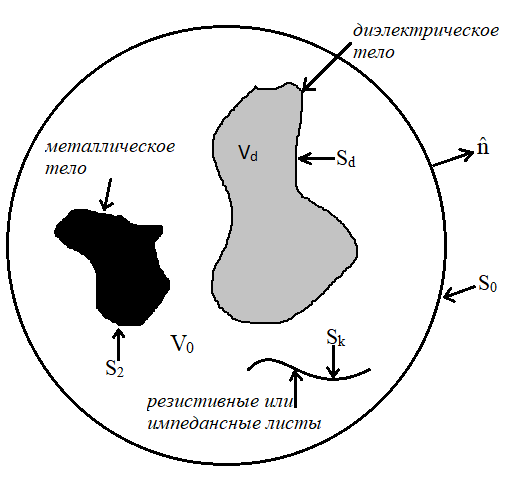
\includegraphics[width=0.6\linewidth]{tes2}
	\caption{}
	\label{fig:tes2}
\end{figure}
\\
Вычислительная область ($ V_{0} $) ограничена поверхностью ($ S_{0} $) и может содержать различные рассеивающие объекты, такие как неоднородные диэлектрики ($ V_{d} $), металлические тела ($ S_{2} $) и резистивные или импедансные листы ($ S_{k} $).\\
Метод конечных элементов позволяет легко моделировать рассеиватели произвольной формы и неоднородные области, не предъявляя жестких требований к их форме, размеру и составу.  \\
Ввиду того, что наш интерес ограничен рассеянием, плотности электрического и магнитного тока будут равны нулю.
С учетом граничных условий на рассеивателе (ях), следует рассмотреть его средневзвешенное значение, дающее так называемую слабую форму векторного волнового уравнения. Для векторной функции $ \vec{E^{'}} $ (1):\\
\begin{center}
	$ 	\iiint\limits_{V_{0}}^{} \left[ \nabla \times \left( \dfrac{1}{\mu_{r}}\nabla \times \vec{E}\right)\cdot \vec{E^{'}} - k_{0}^{2} \epsilon_{r}\vec{E} \cdot \vec{E^{'}} \right]d\upsilon = 0 $
\end{center}
Однако уравнение должно выполняться для каждого из малых объемов, а не в каждой точке $ V_{0} $. Из-за двойного завитка, прямое численное решение уравнения (1) требует расширения $ \vec{E} $ с помощью базисных функций $ S_{0} $ более высокого порядка, и мы также можем получить асимметричную систему. Чтобы избежать этих трудностей и облегчить соблюдение граничных условий, традиционный подход состоит в том, чтобы использовать первую векторную идентичность Грина и переписать формулу: \\
\begin{center}
	$ 	\iiint\limits_{V_{0}}^{} \left[ \dfrac{1}{\mu_{r}}(\nabla \times \vec{E}) \cdot (\nabla \times \vec{E^{'}}) - k_{0}^{2} \epsilon_{r}\vec{E} \cdot \vec{E^{'}} \right]d\upsilon - jk_{0}Z_{0} \oiint (\hat{n} \times \vec{H}) \cdot \vec{E^{'}}ds = 0,$
\end{center}\\
где $ \vec{H} $ - полное магнитное поле, удовлетворяющее уравнению Максвелла $ \nabla \times \vec{E} - jk_{0}Z_{0}\vec{H}  $.\\
Уравнение (№) является слабой формой векторного волнового уравнения. Мы можем решить его численно для $ \vec{E} $, дискретизировав объем $ V_{0} $ и расширив $ \vec{E} $ подходящим, скажем, линейным расширением внутри каждого из подобъемов $V_{e}$. \\
Также необходимо обеспечить соблюдение всех необходимых граничных условий в пределах $V_{0}$ и на $S_{0}$, что подразумевает исключение $\vec{H}$, связав его с $\vec{E}$. \\
Учитывая, что наш интерес заключается в получении рассеяния тела, освещаемого плоской волной, $S_{0}$ служит только в качестве искусственной поверхности для завершения бесконечной вычислительной области. В самом деле, если $S_{0}$ находится далеко от рассеивателя, мы можем тогда вызвать условие излучения Зоммерфельда (2): \\
\begin{center}
	$ jk_{0}Z_{0}\hat{r} \times \vec{H}^{scat} = jk_{0}\hat{r} \times \hat{r} \times \vec{E}^{scat} $ \\
	\begin{center}
связав $ \vec{H} $ и $ \vec{E} $, где $ \hat{r} $ - нормаль к сферической поверхности $ S_{0} $ и \\
		$ \vec{H}^{scat} = \vec{H} - \vec{H}^{inc},\quad \vec{E}^{scat} = \vec{E} - \vec{E}^{inc}$
	\end{center}\\
Обозначим рассеянные поля, связанные с возбуждением плоской волны ($ \vec{E}^{inc} $, $ \vec{H}^{inc} $).
\end{center}
Очевидно, что требование, чтобы $ S_{0} $ располагалась далеко от рассеивателя, значительно увеличивает вычислительный объем, что приводит к непрактично большим системам при дискретизации уравнения. Это побудило к использованию поглощающих граничных условий более высокого порядка, которые можно наносить на поверхность, находящуюся в ближней зоне рассеивателя, без существенного снижения точности решения.Их целью является устранение обратных отражений от $ S_{0} $. \\
Они обеспечивают приблизительную связь между $\vec{E}$ и $\vec{H}$ на поверхности $ S_{0} $, которую мы получаем, предполагая расширение поля в обратных степенях r, радиальное расстояние от центра $S_{0}$. Если поглощающие граничные условия аннулируют первые (2m + 1) обратные степени r, то их называют поглощающие граничные условия m-го порядка.
Поглощающие граничные условия нулевого порядка являются условием излучения Зоммерфельда, приведенным в формуле (2), а их вектор второго порядка имеет вид(3):\\
\begin{center}
	$ -jk_{0}Z_{0}\hat{n} \times \vec{H}^{scat} = jk_{0}\vec{E}_{t}^{scat} + \beta \nabla \times [\hat{n}(\nabla \times \vec{E}^{scat})_{n}] + \beta\nabla_{t} (\nabla \cdot \vec{E}_{t}^{scat})$.
\end{center} \\
В этом уравнении $ \hat{n} $ обозначает внешнюю нормаль к $S_{0}$, $\beta = 1/{2[jk_{0} + (1/r)]}$, а нижние индексы t и n обозначают тангенциальную и нормальную компоненты для $ S_{0} $ соответственно. 
Поглощающие граничные условия (уравнение (3)) были получены для сферической поверхности $ S_{0} $, однако, они хорошо работают, когда $ S_{0} $ является кусочно-плоской, чтобы она лучше соответствовала поверхности рассеивателя.
В этом случае $ \beta $ сводится к $ \beta = 1/(2jk_{0}) $.\\
Точно так же мы можем обобщить уравнение (2) для кусочно-плоских поверхностей, положив $ \hat{r} \rightarrow \hat{n} $.\\
Так же отметим, что, поскольку данные поглощающие граничные условия связывают рассеянные поля, лучше всего переписать формулу (1) в терминах рассеянных полей. Делая так, мы получаем (4): \\
\begin{center}
	$ \iiint\limits_{V_{0}}^{} \left[ \dfrac{1}{\mu_{r}}(\nabla \times \vec{E}^{scat}) \cdot (\nabla \times \vec{E^{'}}) - k_{0}^{2} \epsilon_{r}\vec{E}^{scat} \cdot \vec{E^{'}} \right]d\upsilon + 
	\iint\limits_{S_{0}}^{}  P(\vec{E}^{scat}) \cdot \vec{E^{'}}ds + 
	\iiint\limits_{V_{d}}^{} \left[ \dfrac{1}{\mu_{r}}(\nabla \times \vec{E}^{inc}) \cdot (\nabla \times \vec{E^{'}}) - k_{0}^{2} \epsilon_{r}\vec{E}^{inc} \cdot \vec{E^{'}} \right]d\upsilon + 
	jk_{0}Z_{0}\iint\limits_{S_{d}}^{} \dfrac{1}{\mu_{r}}(\hat{n} \times \vec{H}^{inc}) \cdot \vec{E^{'}}ds = 0, $
\end{center}\\
в котором $P(\vec{E^{scat}})$ равно представлению в правой части уравнения (2), $ V_{d} $ - это объем, занимаемый диэлектриками, а $ S_{d} $ - это поверхность между диэлектрическими интерфейсами. Мы вывели последние два интеграла в формуле (4) снова вызвав первое векторное тождество Грина и отметим, что $ \vec{E^{inc}} $ удовлетворяет волновому уравнению вектора свободного пространства. Очевидно, что (4) относится только к неизвестным $ \vec{E^{scat}} $, и мы можем приступить к его решению.
\section{Тестирование численной схемы}
Приступим к созданию трехмерной модели в программе FreeFem на основе полученных нами выше выражений.  Для этого выберем наиболее подходящий программный способ реализации 3D объектов, а так же сразу определим, что наш объект будет в виде сферы(у которой тут же зададим радиус и другие параметры). 
\\
Возьмем сферическую область, в которой будут рассеиваться волны и заключим в нее наш объект - сферу более маленького радиуса заполненного диэлектриком.
\\
Определим параметры характеризующие наше поле,а именно:
 \\
\begin{flushleft}
	$ \lambda = 10^{-6} $ - длина волны в вакууме в метрах \\
\end{flushleft}
\begin{flushleft}
	$ c = 299792458 $ - скорость света в вакууме \\
\end{flushleft}
\begin{flushleft}
	$ \mu = 4\pi 10^{-7} $ - магнитная проницаемость в свободном пространстве \\
\end{flushleft}
\begin{flushleft}
	$ \varepsilon = \dfrac{\mu}{c^{2}} $ - диэлектрическая проницаемость в свободном пространстве \\
\end{flushleft}
\begin{flushleft}
	$ Z = \sqrt{\dfrac{\mu}{\varepsilon}} $ - импеданс свободного пространства \\
\end{flushleft}
\begin{flushleft}
	$ n = 2 $ - показатель преломления сферы \\
\end{flushleft}
Радиус внутренней сферы (нашего объекта) зададим в 10 раз меньше длины волны принимаемой для расчетов ($ \lambda = 1 $), а радиус внешней сферы в 4 раза больше. Таким образом получим систему состоящую из двух сфер разного радиуса (одна внутри другой), взаимодействие между которыми опиcываются с помощью уравнений полученных ранее. Однако, прежде чем мы это сделаем, определим в программе область расчетов через радиус внутренней сферы, для случаев когда он больше или меньше радиуса применяемого для вычислений полей в ближней и дальней зоне. Необходимость этого заключается в том, что уравнение должно выполняться для каждого из малых объемов, а не в каждой точке, как было сказано ранее.
\\ 
Имея уравнения Лапласа:
\\
\begin{center}
	$ \Delta \vec{E} + k^2\vec{E}=0 $
\end{center}
Опрелелим k для случаев:
\begin{center}
	k = 
	\begin{cases}
		1, & r > a\\
		n, & r < a ,\qquad $ где а - радиус малой сферы $
	\end{cases}
\end{center}
Далее добавим цикл, который ввиду гармонической зависимости от времени будет производить перерасчет данных и выводить результаты на экран, благодаря чему получится наглядная анимированная картина поля. А так же добавим возможность сохранения полученных данных для Matlab.\\
После того, как мы посчитали дифракцию на сфере, перейдем непосредственно к расчету сечения рассеяния и сечения поглощения.\\
Если на рассеивающий элемент падает волна с интенсивностью I(под интенсивностью понимается поток энергии через единичную площадку), то полная рассеянная мощность S будет пропорциональна I. Коэффициент пропорциональности между этими величинами $ \sigma_s $ называется полным сечением рассеяния и имеет размерность площади: \\
\begin{center}
	$ \sigma_s = \dfrac{S}{I} $
\end{center}
Так же введем понятие дифференциального сечения рассеяния
 $ \sigma_d(\theta,\varphi) $. Пусть $ dS(\theta, \varphi) $ - полная мощность, рассеянная в пределах телесного угла d$ \Omega $ в направлении $ (\theta,\varphi) $, тогда:
 \begin{center}
 	$ \sigma_d(\theta,\varphi) = \lim\limits_{d\Omega\rightarrow\infty} \dfrac{dS(\theta, \varphi)}{Id\Omega}. $s
 \end{center}
Приминительно к нашей задаче, это выражение примет вид:
\begin{equation}
\sigma_d(\theta,\varphi) = \lim\limits_{R\rightarrow\infty} \dfrac{R^2 S_r(\theta, \varphi)}{S_i}.
\end{equation}
Здесь вектор Пойнтинга падающей волны
\begin{equation}
{\vec S}_i = \dfrac{1}{2} \left[{\vec E}_i \times {\vec H}^*_i\right],
\end{equation}
радиальная компонента вектора Пойнтинга рассеянных волн
\begin{equation}
{S}_r = \dfrac{1}{2} \left[{\vec E}_s \times {\vec H}^*_s\right] \cdot {\vec \rho}_0
\end{equation}
В нашем случае при расчётах необходимо будет взять значения вектора Пойнтинга рассеянных волн на поверхности с фиксированным значением $R$ (приемлемо, если $R=3\lambda$, т.к. внешняя граница удалена на расстояние $4\lambda$).\\
Наиболее простой способ расчёта $S_r$ через компоненты в декартовой системе координат:
\begin{equation}
{S}_r = S_x \\rm cos(\varphi)\sin(\theta) + S_y \sin(\varphi)\sin(\theta) + S_z \\rm cos(\theta).
\end{equation}
Здесь
\begin{eqnarray}
& S_x = \dfrac{1}{2} \left(E_y H_z^* - E_z H_y^*\right),\nonumber\\
& S_y = \dfrac{1}{2} \left(E_z H_x^* - E_x H_z^*\right),\nonumber\\ & S_z = \dfrac{1}{2} \left(E_x H_y^* - E_y H_x^*\right).
\end{eqnarray}
Предполагается, что поля относятся к рассеянному полю (индеркс $s$ опущен).
Компоненты магнитного поля находим из уравнения Максвелла
\begin{equation}
{\vec H} = \dfrac{i}{k_0} {\rm \rm rot} \vec{E}.
\end{equation}
Полное сечение рассеяния находится как интеграл по полному телесному углу:
\begin{equation}
\sigma_s = \int_{4\pi} \sigma_d d\Omega.
\end{equation}
Сечение поглощения определяется как отношение полной мощности, теряемой первичной волной и преобразующейся в тепло в данной локальной области, к плотности потока энергии(интенсивности) в первичной волне, его находим как:
\begin{equation}
\sigma_a = \left(\int_V \dfrac{1}{2}\omega\varepsilon_0\varepsilon''|{\vec E}|^2 d V\right)/S_i.
\end{equation}
В случае, если падающее поле имеет единичную амплитуду ($|E_i|=1$):
\begin{equation}
\sigma_a = \int_V k \varepsilon''|{\vec E}|^2 d V.
\end{equation}
Здесь интегрирование проводится по области занятой диэлектрическим рассеивателем.\\
Вычисление действительной и мнимой частей диэлектрической проницаемости на основе коэффициента преломления будет выглядеть как:
\begin{equation}
\varepsilon' - i \varepsilon'' = (n'-i n'')^2.
\end{equation}
Отсюда действительная $ \varepsilon' $ и мнимая $ \varepsilon'' $ часть будут соответственно равны:
\begin{equation}
\varepsilon' = (n')^2 - (n'')^2,\quad \varepsilon'' = 2 n'n''.
\end{equation}

\section{Результаты численных расчётов}
Ниже приведены результаты численных расчётов сечения рассеяния и сечения поглощения для рассеивателей, состоящих из одного шара, пяти и семнадцати. Шары заполнены золотом, серебром, либо медью.
\begin{figure}[h!]
	\centering
	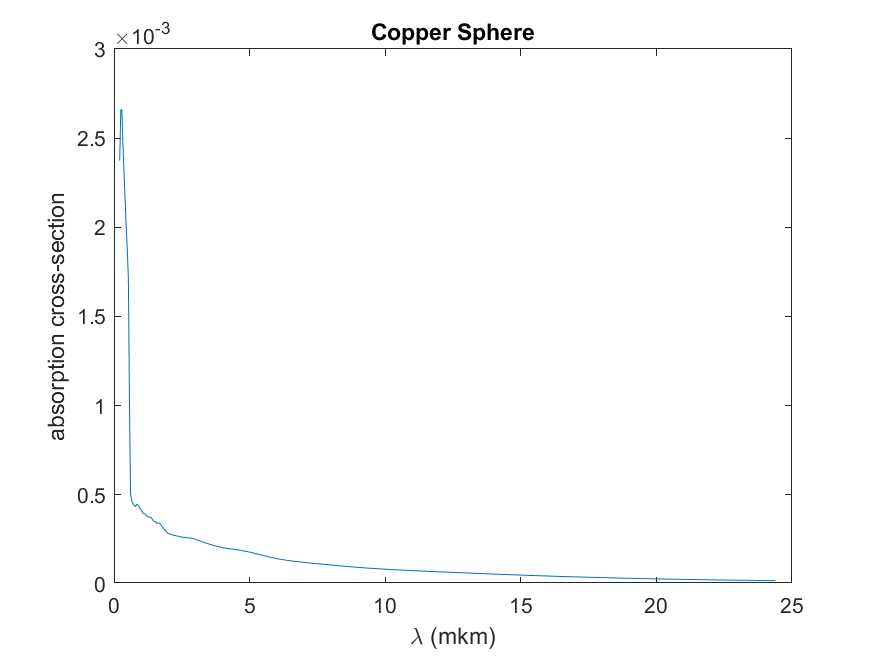
\includegraphics[width=0.5\linewidth]{singleCopperSphereAbsorptionSection}
	\caption{Поглощение на одиночной медной сфере}
	\label{fig:singleCopperSphereAbsorptionSection}
\end{figure} \\
\begin{figure}[h!]
	\centering
	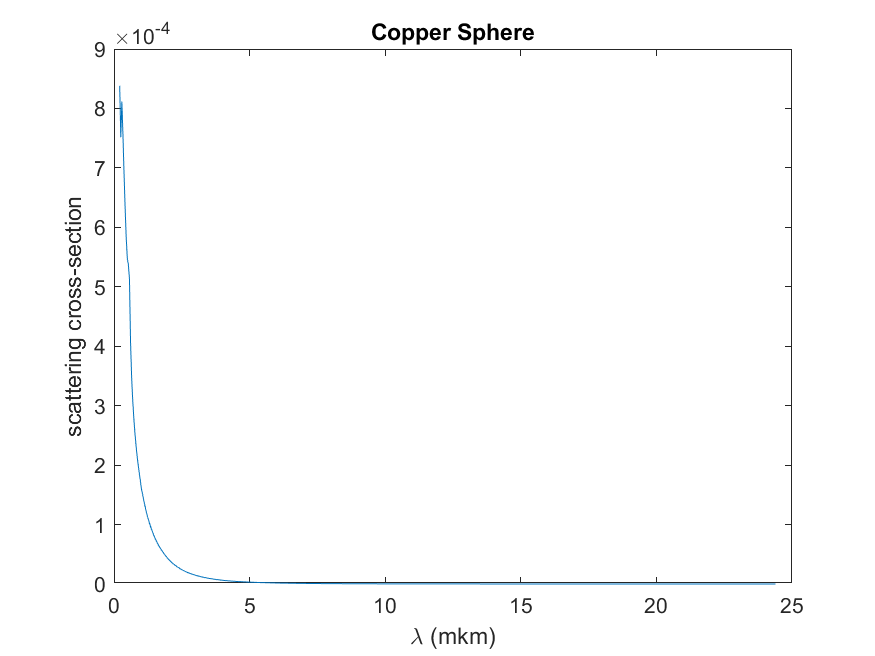
\includegraphics[width=0.5\linewidth]{singleCopperSphereCrossSection}
	\caption{Рассеяние на одиночной медной сфере}
	\label{fig:singleCopperSphereCrossSection}
\end{figure} \\
\begin{figure}[h!]
	\centering
	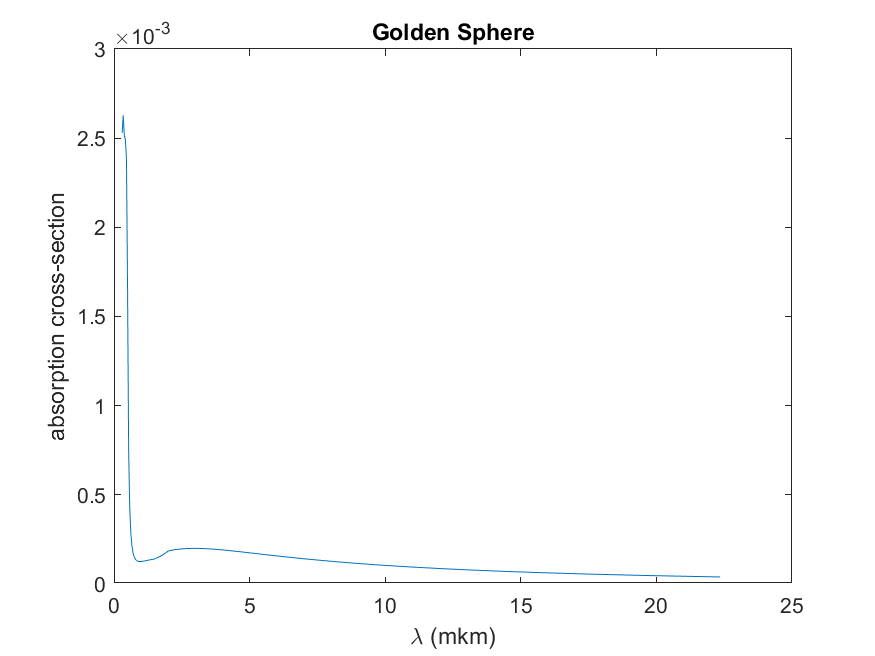
\includegraphics[width=0.5\linewidth]{singleGoldSphereAbsorptionSection}
	\caption{Поглощение на одиночной золотой сфере}
	\label{fig:singleGoldSphereAbsorptionSection}
\end{figure} \\
\begin{figure}[h!]
	\centering
	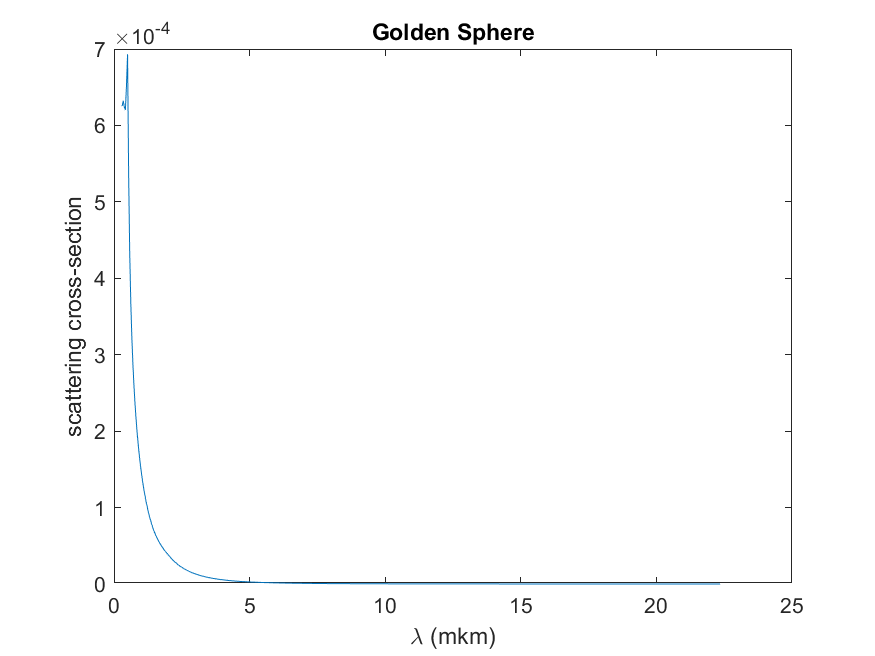
\includegraphics[width=0.5\linewidth]{singleGoldSphereCrossSection}
	\caption{Рассеяние на одиночной золотой сфере}
	\label{fig:singleGoldSphereCrossSection}
\end{figure} \\
\begin{figure}[h!]
	\centering
	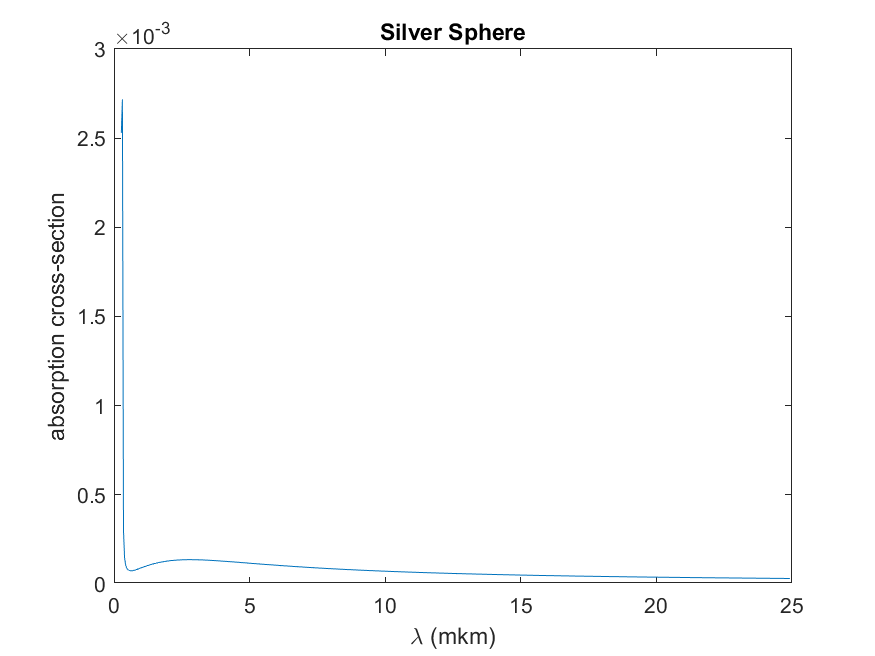
\includegraphics[width=0.5\linewidth]{singleSilverSphereAbsorptionSection}
	\caption{Поглощение на одиночной серебряной сфере}
	\label{fig:singleSilverSphereAbsorptionSection}
\end{figure} \\
\begin{figure}[h!]
	\centering
	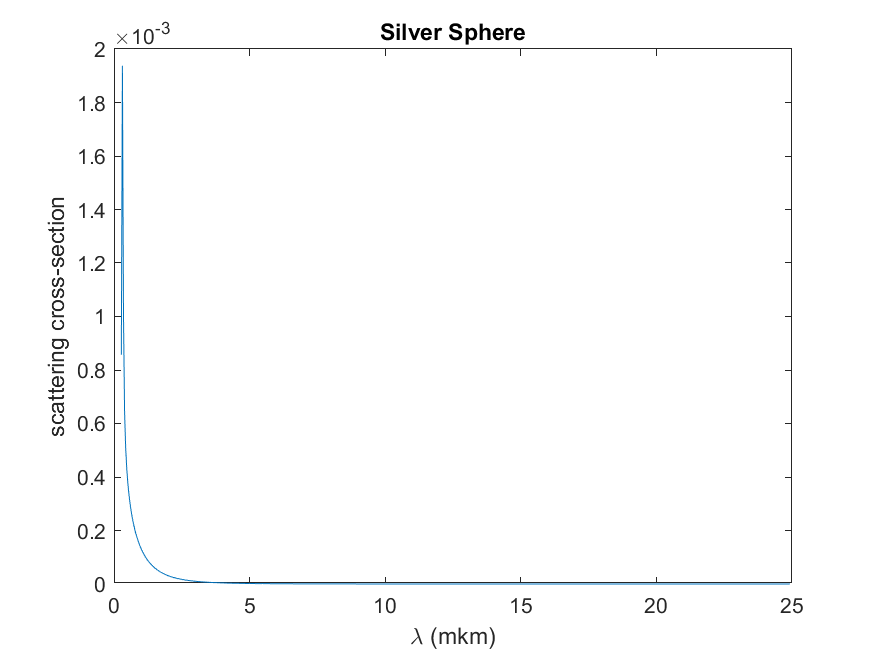
\includegraphics[width=0.5\linewidth]{singleSilverSphereCrossSection}
	\caption{Рассеяние на одиночной серебряной сфере}
	\label{fig:singleSilverSphereCrossSection}
\end{figure} \\
\begin{figure}[h!]
	\centering
	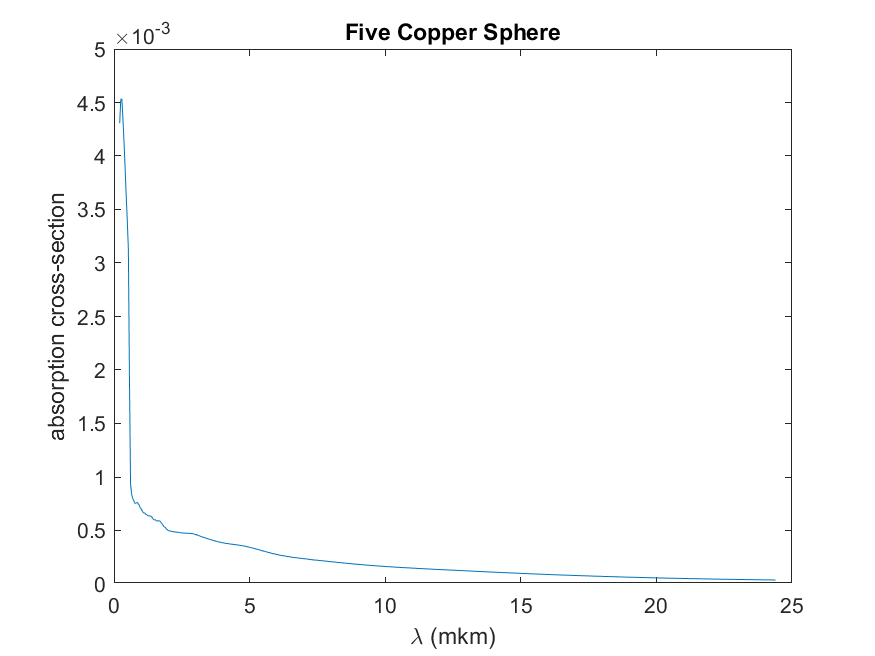
\includegraphics[width=0.5\linewidth]{fiveCopperSphereAbsorptionSection}
	\caption{Поглощение на 5 медных сферах}
	\label{fig:fiveCopperSphereAbsorptionSection}
\end{figure} \\
\begin{figure}[h!]
	\centering
	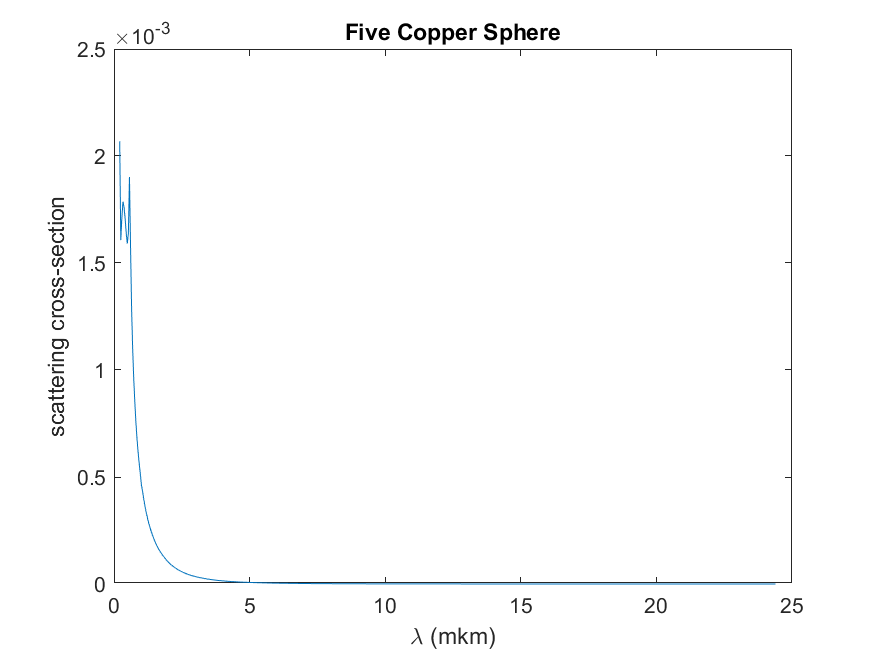
\includegraphics[width=0.5\linewidth]{fiveCopperSphereCrossSection}
	\caption{Рассеяние на 5 медных сферах}
	\label{fig:fiveCopperSphereCrossSection}
\end{figure} \\
\begin{figure}[h!]
	\centering
	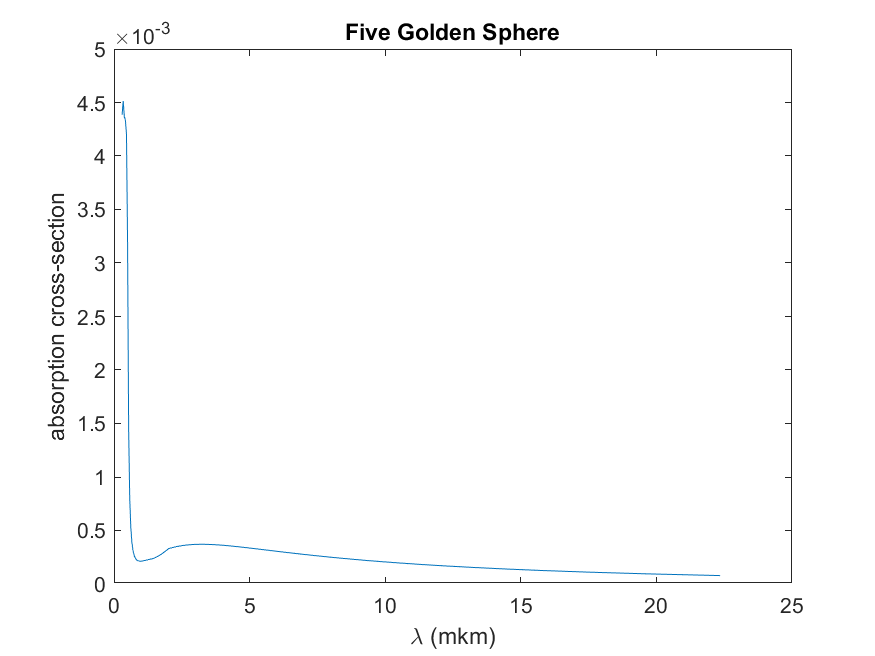
\includegraphics[width=0.5\linewidth]{fiveGoldSphereAbsorptionSection}
	\caption{Поглощение на 5 золотых сферах}
	\label{fig:fiveGoldSphereAbsorptionSection}
\end{figure} \\
\begin{figure}[h!]
	\centering
	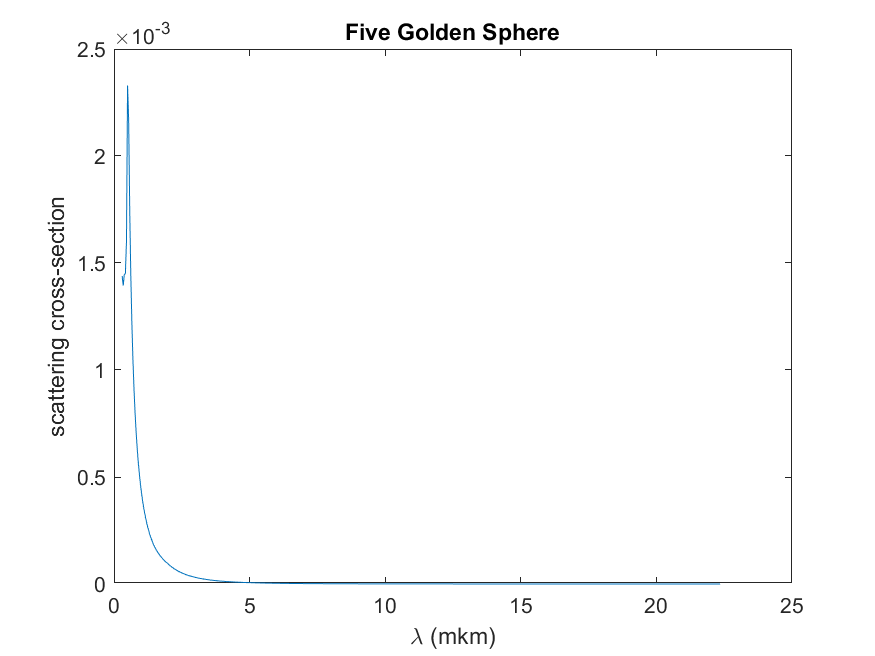
\includegraphics[width=0.5\linewidth]{fiveGoldSphereCrossSection}
	\caption{Рассеяние на 5 золотых сферах}
	\label{fig:fiveGoldSphereCrossSection}
\end{figure} \\
\begin{figure}[h!]
	\centering
	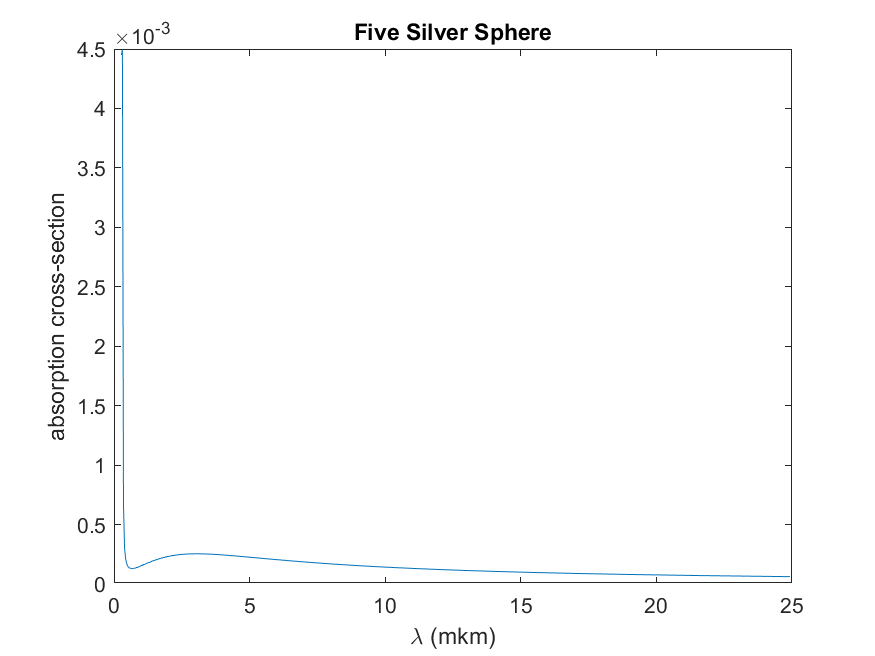
\includegraphics[width=0.5\linewidth]{fiveSilverSphereAbsorptionSection}
	\caption{Поглощение на 5 серебряных сферах}
	\label{fig:fiveSilverSphereAbsorptionSection}
\end{figure} 
\begin{figure}[h!]
	\centering
	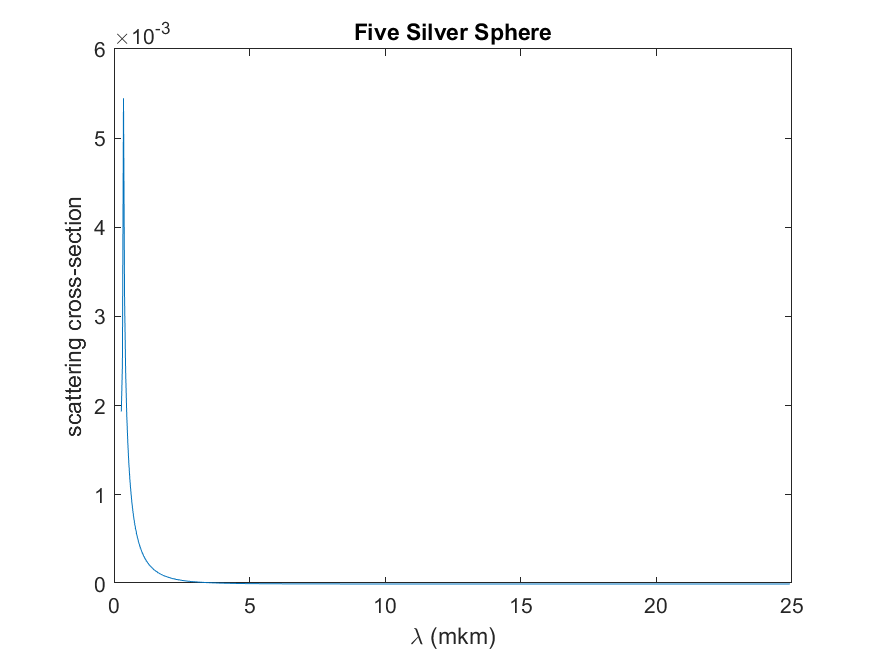
\includegraphics[width=0.5\linewidth]{fiveSilverSphereCrossSection}
	\caption{Рассеяние на 5 серебряных сферах}
	\label{fig:fiveSilverSphereCrossSection}
\end{figure} \\
\begin{figure}[h!]
	\centering
	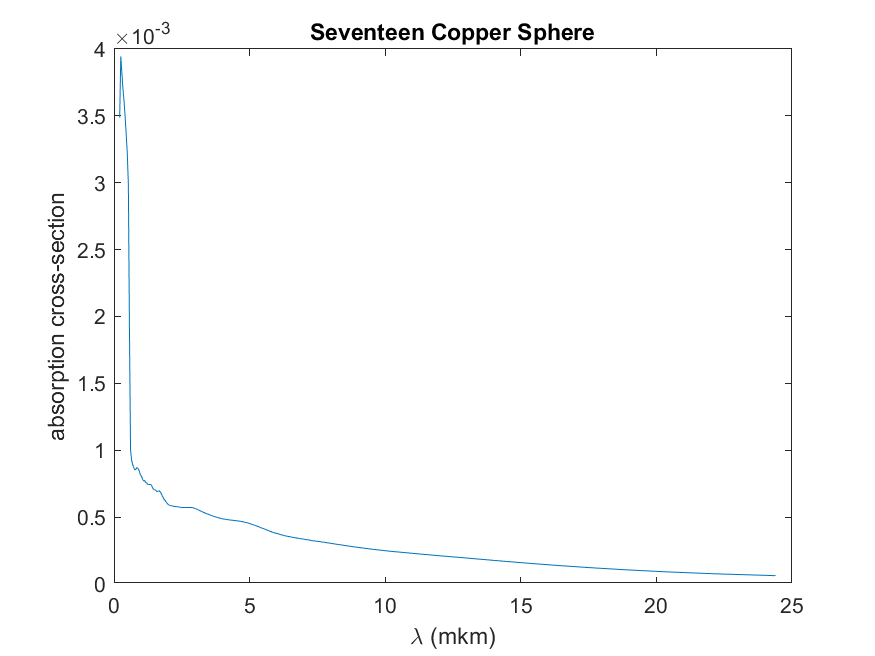
\includegraphics[width=0.5\linewidth]{seventeenCopperSphereAbsorptionSection}
	\caption{Поглощение на 17 медных сферах}
	\label{fig:seventeenCopperSphereAbsorptionSection}
\end{figure} 
\begin{figure}[h!]
	\centering
	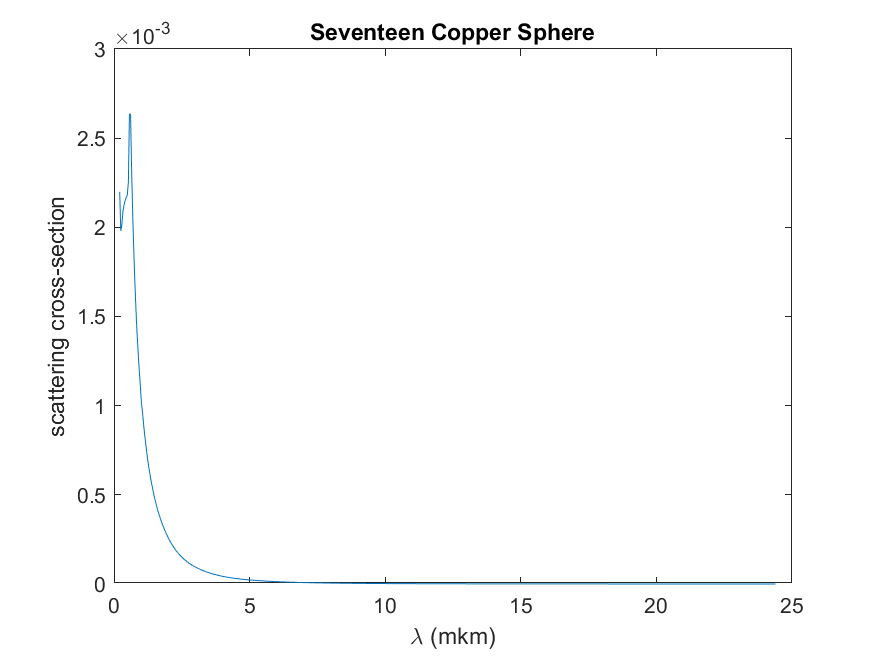
\includegraphics[width=0.5\linewidth]{seventeenCopperSphereCrossSection}
	\caption{Рассеяние на 17 медных сферах}
	\label{fig:seventeenCopperSphereCrossSection}
\end{figure} \\
\begin{figure}[h!]
	\centering
	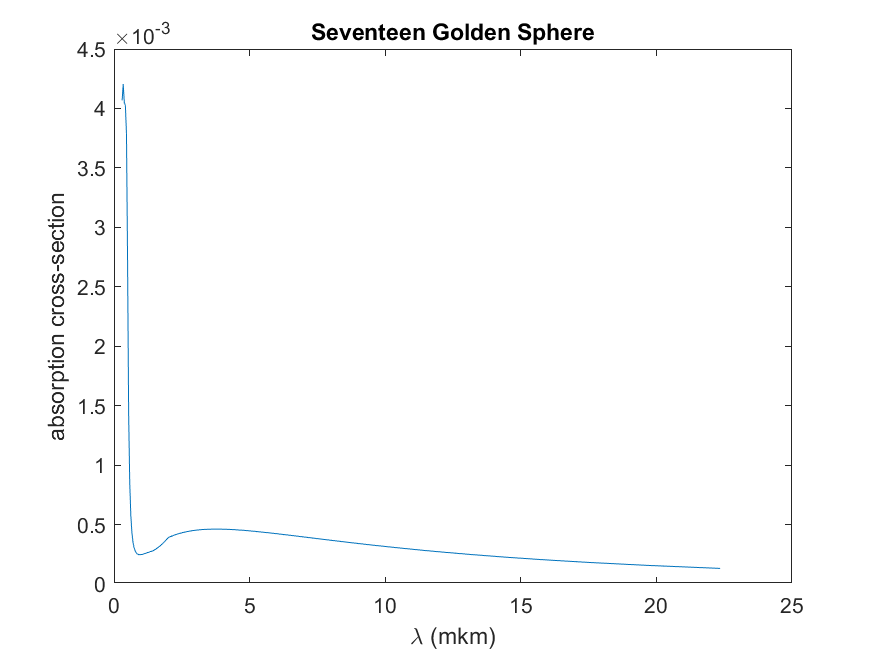
\includegraphics[width=0.5\linewidth]{seventeenGoldSphereAbsorptionSection}
	\caption{Поглощение на 17 золотых сферах}
	\label{fig:seventeenGoldSphereAbsorptionSection}
\end{figure} 
\begin{figure}[h!]
	\centering
	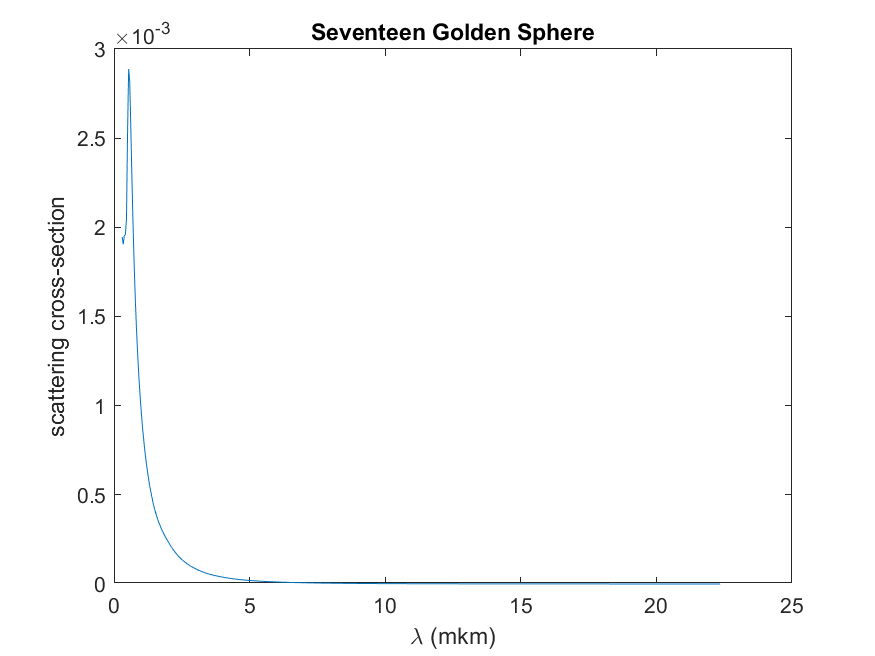
\includegraphics[width=0.5\linewidth]{seventeenGoldSphereCrossSection}
	\caption{Рассеяние на 17 золотых сферах}
	\label{fig:seventeenGoldSphereCrossSection}
\end{figure} \\
\begin{figure}[h!]
	\centering
	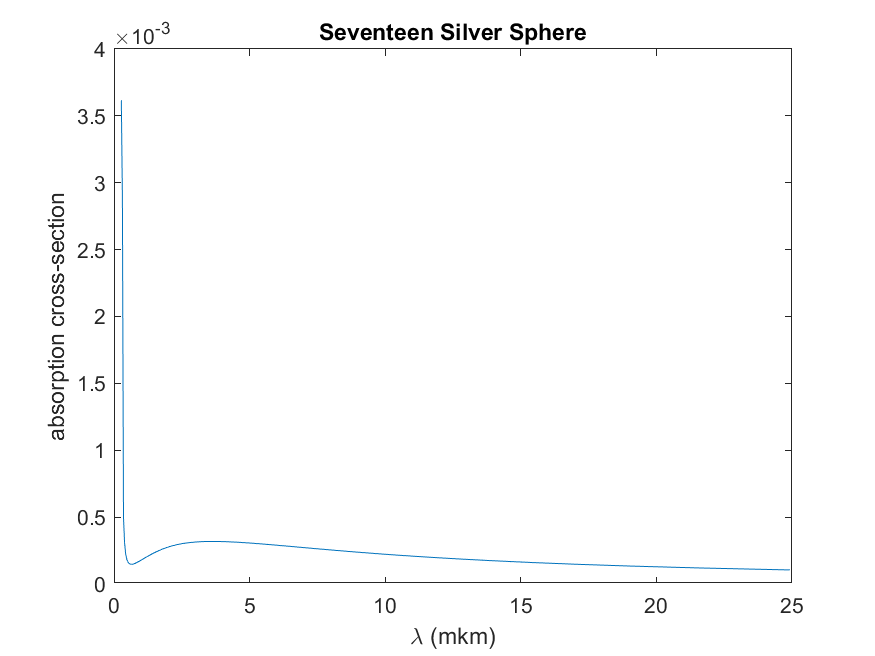
\includegraphics[width=0.5\linewidth]{seventeenSilverSphereAbsorptionSection}
	\caption{Поглощение на 17 серебряных сферах}
	\label{fig:seventeenSilverSphereAbsorptionSection}
\end{figure} 
\begin{figure}[h!]
	\centering
	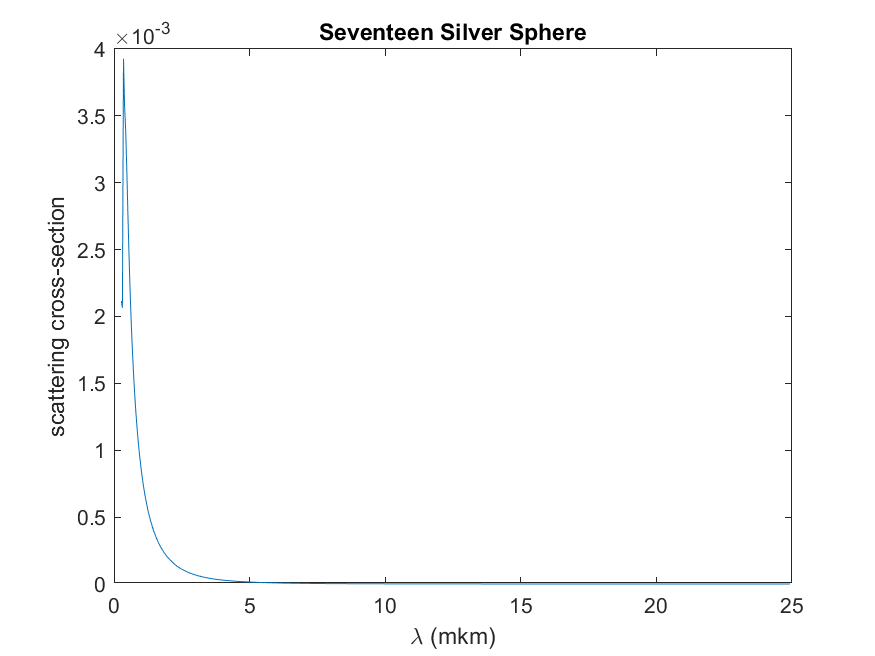
\includegraphics[width=0.5\linewidth]{seventeenSilverSphereCrossSection}
	\caption{Рассеяние на 17 серебряных сферах}
	\label{fig:seventeenSilverSphereCrossSection}
\end{figure} \\
% Глава 2
%\input{2}

% Заключение
\conclusion
В настоящей работе рассмотрены такие интегральные характеристики рассеивателей при рассеянии на них плоской волны как сечение рассеяния и сечение поглощения, при разной геометрии объекта, материалов, составляющих элементы, и частоты падающего излучения. Получены выражения для рассеяния плоской электромагнитной волны на одиночном цилиндре численным и точным методом. Рассмотрена задача дифракции одиночной сферы используя метод конечных элементов. Были протестированы полученные численные схемы с помощью программы FreeFem. Установлены зависимости частот от длин волн при рассеянии на разных типах и колличествах сфер. А именно, получены графики для поглощения и рассеяния электромагнитной волны на одиночной медной,серебряной,золотой сфере. Их первой итерации состоящей из 5 сфер, а так же для второй инетарции состоящей из 17 сфер. Было показано, что некоторые графики имеют схожую зависимость с гиперболическим косекансом. Установлено, что с ростом частоты происходит уменьшение диапазона длин волн как для сечения рассеяния, так и для сечения поглощения. Увеличении элементов рассеивателя приводит к расширению диапазона длин волн, однако с каждой итерацией это изменение становится менее значительно. Было показано, как именно выбор материала может повлиять на максимальную частоту и диапазон длин волн. 


\newpage
% Приложения
\appendix
\chapter{Код программы для расчета сечений рассеяния и поглощения, структуры поля в случае рассеяния плоской волны на фрактальном объекте}

\begin{lstlisting}[language=C]
verbosity=1;
load "msh3"
load "tetgen"
load "medit"
include "MeshSurface.idp"
include "ffmatlib.idp"


real c0 = 299792458;        // speed of light in vacuum
real mue0 = 4.*pi*1e-7;     // Permeability of free space
real eps0 = 1./c0^2/mue0;   // Permittivity of free space
real Z0 = sqrt(mue0/eps0);  // Impedance of free space

real    lambda0 = 10e-6;        // vacuum wavelength (in m)
complex ns    = 10.- 1i*70.;   // sphere refractive index (complex)
ns = 2.;
// ns = 1.; // test - uniform media

real lambda = 1.;        // vacuum wavelength (in 10*1e-6 m)
real radiusOfInnerSpher = lambda / 10.;

real k0 = 2.* pi / lambda;
complex k2 = k0 * ns;
real w = c0 * 2.* pi / lambda0;
real alpha=1; 	//penalty term

meshS ThHex;
real volumetet;  // use in tetg.

//real step = 0.2/radiusOfInnerSpher;
real step = lambda / 20.;
//cout << "step = "<< step << endl;

real volumetetIn = (step^3)/6.;  
//step = lambda / 2;

//////////////////////////////////////////////////////////////////////////////////////////////
///////////////////////////// creating an inner spheres ///////////////////////////////////////
////// zero iteration
meshS ThInnerSphere; //
ThInnerSphere = Sphere(radiusOfInnerSpher,    step,   11, -1);
//medit("Scatterer", ThInnerSphere,wait=1);
/////////////////////////// first iteration ///////////////////////////////////////////////////

meshS ThInnerSphere2 = Sphere(radiusOfInnerSpher/2, step/2, 13, -1);
real ddx = radiusOfInnerSpher + radiusOfInnerSpher/2;
ThInnerSphere2 = movemeshS(ThInnerSphere2,transfo=[x + ddx,y,z]);
meshS ThInnerSphere3 = Sphere(radiusOfInnerSpher/2, step/2, 14, -1);
ThInnerSphere3 = movemeshS(ThInnerSphere3,transfo=[x - ddx,y,z]);

meshS ThInnerSphere4 = Sphere(radiusOfInnerSpher/2, step/2, 15, -1);
ThInnerSphere4 = movemeshS(ThInnerSphere4,transfo=[x,y + ddx,z]);
meshS ThInnerSphere5 = Sphere(radiusOfInnerSpher/2, step/2, 16, -1);
ThInnerSphere5 = movemeshS(ThInnerSphere5,transfo=[x,y - ddx,z]);
//medit("Bounday mesh",ThInnerSphere,wait=1);


/////////////////////////////////////////////////////////////////////////////
meshS ThS =  ThInnerSphere + ThInnerSphere2 + ThInnerSphere3 + ThInnerSphere4 + ThInnerSphere5;
//medit("Bounday mesh",ThS,wait=1);

////////////////// second iteration //////////////////////////////////////////////////////////
meshS ThInnerSphere21 = Sphere(radiusOfInnerSpher/4, step/4, 17, -1);
meshS ThInnerSphere22 = Sphere(radiusOfInnerSpher/4, step/4, 18, -1);
meshS ThInnerSphere23 = Sphere(radiusOfInnerSpher/4, step/4, 19, -1);
real ddy = radiusOfInnerSpher/2. + radiusOfInnerSpher/4.;
ThInnerSphere21 = movemeshS(ThInnerSphere21,transfo=[x + ddx,y + ddy,z]);
ThInnerSphere22 = movemeshS(ThInnerSphere23,transfo=[x + ddx + ddy,y,z]);
ThInnerSphere23 = movemeshS(ThInnerSphere23,transfo=[x + ddx,y - ddy,z]);

ThS =  ThS + ThInnerSphere21 + ThInnerSphere23 + ThInnerSphere22;


meshS ThInnerSphere31 = Sphere(radiusOfInnerSpher/4, step/4, 20, -1);
meshS ThInnerSphere32 = Sphere(radiusOfInnerSpher/4, step/4, 21, -1);
meshS ThInnerSphere33 = Sphere(radiusOfInnerSpher/4, step/4, 22, -1);
ThInnerSphere31 = movemeshS(ThInnerSphere31,transfo=[x - ddx,y + ddy,z]);
ThInnerSphere32 = movemeshS(ThInnerSphere33,transfo=[x - ddx - ddy,y,z]);
ThInnerSphere33 = movemeshS(ThInnerSphere33,transfo=[x - ddx,y - ddy,z]);

ThS =  ThS + ThInnerSphere31 + ThInnerSphere33 + ThInnerSphere32;


meshS ThInnerSphere41 = Sphere(radiusOfInnerSpher/4, step/4, 23, -1);
meshS ThInnerSphere42 = Sphere(radiusOfInnerSpher/4, step/4, 24, -1);
meshS ThInnerSphere43 = Sphere(radiusOfInnerSpher/4, step/4, 25, -1);
ThInnerSphere41 = movemeshS(ThInnerSphere41,transfo=[x,y + ddx + ddy,z]);
ThInnerSphere42 = movemeshS(ThInnerSphere43,transfo=[x + ddy,y + ddx,z]);
ThInnerSphere43 = movemeshS(ThInnerSphere43,transfo=[x - ddy,y + ddx,z]);

ThS =  ThS + ThInnerSphere41 + ThInnerSphere43 + ThInnerSphere42;


meshS ThInnerSphere51 = Sphere(radiusOfInnerSpher/4, step/4, 26, -1);
meshS ThInnerSphere52 = Sphere(radiusOfInnerSpher/4, step/4, 27, -1);
meshS ThInnerSphere53 = Sphere(radiusOfInnerSpher/4, step/4, 28, -1);
ThInnerSphere51 = movemeshS(ThInnerSphere51,transfo=[x,y - ddx - ddy,z]);
ThInnerSphere52 = movemeshS(ThInnerSphere53,transfo=[x + ddy,y - ddx,z]);
ThInnerSphere53 = movemeshS(ThInnerSphere53,transfo=[x - ddy,y - ddx,z]);

ThS =  ThS + ThInnerSphere51 + ThInnerSphere53 + ThInnerSphere52;
medit("Scatterer",ThS,wait=1);

//////////////////////////////////////////////////////////////////////////////////////////////
///////////////////////////// creating an outer sphere ///////////////////////////////////////
step = lambda / 2.;
volumetet = (step^3)/6.;  
meshS ThOuterSphere; // 
real radiusOfOuterSphere = 4.* lambda;
ThOuterSphere = Sphere(radiusOfOuterSphere, step,12,1);

meshS ThVirtualSphere; // 
real radiusOfVirtualSphere = 3.* lambda;
ThVirtualSphere = Sphere(radiusOfVirtualSphere, step, 123, -1);
ThS =  ThS + ThOuterSphere + ThVirtualSphere;
medit("3td iteration",ThS,wait=1);
/////////////////////////////////////////////////////////////////////////////

real[int] domaine  = [0,0,radiusOfOuterSphere-0.1,1,volumetet,0.,0,0.,2,volumetetIn,0.,0,radiusOfVirtualSphere-0.1,3,volumetet,ddx,0,0.,4,volumetetIn,-ddx,0,0,5,volumetetIn,0,ddx,0,6,volumetetIn,0,-ddx,0,7,volumetetIn, ddx,ddy,0,8,volumetetIn,ddx,-ddy,0.,9,volumetetIn,ddx+ddy,0,0.,10,volumetetIn,-ddx,ddy,0,11,volumetetIn,-ddx,-ddy,0,12,volumetetIn,-ddx-ddy,0,0,13,volumetetIn, 0,ddx+ddy,0,14,volumetetIn, -ddy,ddx,0,15,volumetetIn, ddy,ddx,0,16,volumetetIn, 0, -ddx-ddy,0,17,volumetetIn, ddy,-ddx,0,18,volumetetIn, -ddy, -ddx,0,19,volumetetIn];
//
mesh3 Th = tetg(ThS,switch="pqaAAYYQ",nbofregions=19,regionlist=domaine);
// Tetrahelize the interior of the cube with tetgen
medit("3td iteration",Th,wait=1);

fespace Ph(Th,P03d);
fespace Vh(Th,P1);
Ph reg = region;           // function that returns region number of a point XY
Ph inReg  = sqrt(x^2.+y^2. + z^2.) < radiusOfInnerSpher;  //subdomains for inside the sratterer
Ph outReg = sqrt(x^2.+y^2. + z^2.) > radiusOfInnerSpher;  //subdomains for outside the scatterer
Vh dd = inReg;

//plot(dd,wait=1,value=1);

cout << "  centre = " << reg(0,0,0) << endl;
cout << " virtual = " << reg(0,0,radiusOfVirtualSphere-0.1) << endl;
cout << " exterieur = " << reg(0,0,radiusOfOuterSphere-0.1) << endl;

macro Grad(u) [dx(u),dy(u),dz(u)] // EOM
macro Curl(ux, uy, uz)[dy(uz)-dz(uy), dz(ux)-dx(uz), dx(uy)-dy(ux)]// EOM
macro Div(ux, uy, uz)[dx(ux) + dy(uy) + dz(uz)]// EOM
macro CrossN(ux, uy, uz)[uy*N.z-uz*N.y, uz*N.x-ux*N.z, ux*N.y-uy*N.x]// EOM
macro Curlabs(ux, uy, uz)[abs(dy(uz)-dz(uy)), abs(dz(ux)-dx(uz)), abs(dx(uy)-dy(ux))]// EOM

real t = 0.;

Vh<complex> Hz, hz;
Vh<complex> Ex1 = exp(- 1i* k0 * z);
Vh <complex> Ez,ez,Ey,ey,Ex,ex,Hy,Sx,Sy,Sz,Sr,Hx,Si,SigmD;
Vh <complex> N0;


func complex Eps() {
if (Th(x,y,z).region == Th(0.0,0.0,0.0).region || Th(x,y,z).region == Th(ddx,0.0,0.0).region || Th(x,y,z).region == Th(-ddx,0.0,0.0).region || Th(x,y,z).region == Th(0.0, ddx, 0.0).region || Th(x,y,z).region == Th(0.0,-ddx,0.0).region ||
Th(x,y,z).region == Th(ddx,ddy,0.0).region || Th(x,y,z).region == Th(ddx+ddy,0.0,0.0).region || Th(x,y,z).region == Th(ddx,-ddy,0.0).region ||
Th(x,y,z).region == Th(-ddx,ddy,0.0).region || Th(x,y,z).region == Th(-ddx-ddy,0.0,0.0).region || Th(x,y,z).region == Th(-ddx,-ddy,0.0).region ||
Th(x,y,z).region == Th(0.0,ddx+ddy,0.0).region || Th(x,y,z).region == Th(ddy,ddx,0.0).region || Th(x,y,z).region == Th(-ddy,ddx,0.0).region ||
Th(x,y,z).region == Th(0.0,-ddx-ddy,0.0).region || Th(x,y,z).region == Th(ddy,-ddx,0.0).region || Th(x,y,z).region == Th(-ddy,-ddx,0.0).region)
return ns^2;
else 
return 1.0;
}

func real InInner() {
if (Th(x,y,z).region == Th(0.0,0.0,0.0).region || Th(x,y,z).region == Th(ddx,0.0,0.0).region || Th(x,y,z).region == Th(-ddx,0.0,0.0).region || Th(x,y,z).region == Th(0.0, ddx, 0.0).region || Th(x,y,z).region == Th(0.0,-ddx,0.0).region ||
Th(x,y,z).region == Th(ddx,ddy,0.0).region || Th(x,y,z).region == Th(ddx+ddy,0.0,0.0).region || Th(x,y,z).region == Th(ddx,-ddy,0.0).region ||
Th(x,y,z).region == Th(-ddx,ddy,0.0).region || Th(x,y,z).region == Th(-ddx-ddy,0.0,0.0).region || Th(x,y,z).region == Th(-ddx,-ddy,0.0).region ||
Th(x,y,z).region == Th(0.0,ddx+ddy,0.0).region || Th(x,y,z).region == Th(ddy,ddx,0.0).region || Th(x,y,z).region == Th(-ddy,ddx,0.0).region ||
Th(x,y,z).region == Th(0.0,-ddx-ddy,0.0).region || Th(x,y,z).region == Th(ddy,-ddx,0.0).region || Th(x,y,z).region == Th(-ddy,-ddx,0.0).region)
return 1.;
else 
return 0.;
}


//////////////////// calculation of the scattered field /////////////////////  
problem MaxwellEquationsForH3D([Ex,Ey,Ez],[ex,ey,ez]) =
int3d(Th)(Curl(ex,ey,ez)'*Curl(Ex,Ey,Ez))
- int3d(Th)(k0^2 * Eps() * [ex,ey,ez]'*[Ex,Ey,Ez])
+ int2d(Th,11)( 1i*k0 * ( ez * N.x - ex * N.z) * Ex1)
+ int2d(Th,13)( 1i*k0 * ( ez * N.x - ex * N.z) * Ex1)
+ int2d(Th,14)( 1i*k0 * ( ez * N.x - ex * N.z) * Ex1)
+ int2d(Th,15)( 1i*k0 * ( ez * N.x - ex * N.z) * Ex1)
+ int2d(Th,16)( 1i*k0 * ( ez * N.x - ex * N.z) * Ex1)

+ int2d(Th,17)( 1i*k0 * ( ez * N.x - ex * N.z) * Ex1)
+ int2d(Th,18)( 1i*k0 * ( ez * N.x - ex * N.z) * Ex1)
+ int2d(Th,19)( 1i*k0 * ( ez * N.x - ex * N.z) * Ex1)
+ int2d(Th,20)( 1i*k0 * ( ez * N.x - ex * N.z) * Ex1)
+ int2d(Th,21)( 1i*k0 * ( ez * N.x - ex * N.z) * Ex1)
+ int2d(Th,22)( 1i*k0 * ( ez * N.x - ex * N.z) * Ex1)
+ int2d(Th,23)( 1i*k0 * ( ez * N.x - ex * N.z) * Ex1)
+ int2d(Th,24)( 1i*k0 * ( ez * N.x - ex * N.z) * Ex1)
+ int2d(Th,25)( 1i*k0 * ( ez * N.x - ex * N.z) * Ex1)
+ int2d(Th,26)( 1i*k0 * ( ez * N.x - ex * N.z) * Ex1)
+ int2d(Th,27)( 1i*k0 * ( ez * N.x - ex * N.z) * Ex1)
+ int2d(Th,28)( 1i*k0 * ( ez * N.x - ex * N.z) * Ex1)
+ int2d(Th,12)(-1i*k0 * ((ex * N.x + ey * N.y + ez * N.z)*(Ex * N.x + Ey * N.y + Ez * N.z) - (Ex * ex + Ey * ey + Ez * ez)))
;

MaxwellEquationsForH3D;

real R = 3. * lambda;
Vh Phi = atan(y/x);
Vh teta = acos(z / sqrt(x^2 + y^2 + z^2));
complex E = 1.;
Hx = 1i/k0 * (dy(Ez)-dz(Ey));
Hy = 1i/k0 * (dz(Ex)-dx(Ez));
Hz = 1i/k0 * (dx(Ey)-dy(Ex));
Sx = 1./2. * (Ey*conj(Hz) - Ez*conj(Hy));
Sy = 1./2. * (Ez*conj(Hx) - Ex*conj(Hz));
Sz = 1./2. * (Ex*conj(Hy) - Ey*conj(Hx));
Sr = Sx * cos(Phi) * sin(teta) + Sy * sin(Phi) * sin (teta) + Sz * cos(teta);
Vh R2 = x^2+y^2+z^2;
Si = 1.;

SigmD = R2 * Sr/Si;

complex sigmaTotal = (int2d(Th, 123)(R2 * Sr));
cout << "sigmaTotal = " << sigmaTotal << endl;

real sigmaT = (int2d(Th, 123)(R2 * real(Sr)));
cout << "sigmaT = " << sigmaT << endl;

Vh <complex> EpsI; // EpsI - epsilon imaginary

EpsI = 2*real(ns)*imag(ns);

complex sigmaAbsorption = (int3d(Th) ( InInner() *(k0 * EpsI * (Ex * conj(Ex)  +   Ey * conj(Ey) +   Ez * conj(Ez))))); 
cout << "sigmaAbsorption = " << sigmaAbsorption << endl;		 


Vh realHz, realEy, realEx, realEx1;
Vh<complex> HzInTime = 0.;
Vh<complex> Ex1InTime = 0.;
Vh<complex> E0=1.;
Ex1InTime = Ex + (1. - InInner()) * Ex1;
realEx1 = real(Ex1InTime);

cout << "k0 = " << k0 << endl;

//Ex1InTime = outReg + 1i *0;

///// save for the matlab
savemesh(Th,"diffractionSInS3d.mesh");
ffSaveVh(Th,Vh,"diffractionSInS3d_vh.txt");
ffSaveData(Ey,"diffractionSInS3d_Ey.txt");
ffSaveData(Ex1InTime,"diffractionSInS3d_Ex.txt");
ffSaveData(SigmD,"diffractionSInS3d_SigmaD.txt");
/////////////////////////
Ex1InTime = Ex + (1. - InInner()) * Ex1;
realEx1 = real(Ex1InTime);
plot(realEx1,wait=1,value=1);

real dt = 2.* pi/ w / 20;
for (int i=1; i < 100; i++)
{
t = dt * i;
cout<< "Time is" << t << endl;

Ex1InTime = Ex * exp (1i*(w*t)) + (1. - InInner()) * (Ex1 * exp (1i*(w*t)));
realEx1 = real(Ex1InTime);

plot(realEx1,wait=0,value=1);
}
\end{lstlisting}
\chapter{Код программы расчета сечений рассеяния и поглощения в зависимости от длины волны}

\begin{lstlisting}[language=C]
verbosity=1;
load "msh3"
load "tetgen"
load "medit"
include "MeshSurface.idp"
include "ffmatlib.idp"

real c0 = 299792458;        // speed of light in vacuum
real mue0 = 4.*pi*1e-7;     // Permeability of free space
real eps0 = 1./c0^2/mue0;   // Permittivity of free space
real Z0 = sqrt(mue0/eps0);  // Impedance of free space

real    lambda0 = 10e-6;        // vacuum wavelength (in m)
complex ns    = 10.- 1i*70.;   // sphere refractive index (complex)
ns = 2.;
// ns = 1.; // test - uniform media
///// gold media
matrix<real> sortGoldWavelengthNK = [[0.3,1.562,1.827],[0.34,1.65,1.784],[0.38,1.55,1.832],[0.42,1.533,1.85],
[0.46,1.399,1.774],[0.5,0.8181,1.745],[0.54,0.3897,2.298],[0.58,0.2553,2.803],
[0.62,0.1916,3.237],[0.66,0.157,3.632],[0.7,0.138,4.002],[0.74,0.1282,4.354],
[0.78,0.1243,4.694],[0.82,0.1241,5.023],[0.86,0.1266,5.345],[0.9,0.1309,5.66],
[0.94,0.1367,5.97],[0.98,0.1435,6.276],[1.02,0.1511,6.579],[1.06,0.1594,6.878],
[1.1,0.1683,7.175],[1.14,0.1776,7.47],[1.18,0.1874,7.762],[1.22,0.1975,8.053],
[1.26,0.2079,8.342],[1.3,0.2187,8.63],[1.34,0.2297,8.916],[1.45,0.2611,9.698],
[1.49,0.2747,9.952],[1.53,0.2891,10.2],[1.57,0.3042,10.45],[1.61,0.3201,10.7],
[1.65,0.3369,10.94],[1.69,0.3546,11.18],[1.73,0.3733,11.42],
[1.77,0.3931,11.65],[1.81,0.414,11.88],[1.85,0.4361,12.11],[1.89,0.4595,12.34],
[1.93,0.4842,12.57],[1.97,0.5104,12.79],[2.007,0.5345,13],[2.045,0.5544,13.25],
[2.084,0.5754,13.51],[2.125,0.5977,13.78],[2.168,0.6213,14.06],
[2.205,0.6421,14.3],[2.243,0.6639,14.55],[2.282,0.6869,14.8],
[2.323,0.711,15.07],[2.365,0.7365,15.35],[2.409,0.7634,15.63],
[2.446,0.786,15.87],[2.483,0.8096,16.11],[2.522,0.8342,16.36],
[2.562,0.86,16.62],[2.603,0.8871,16.89],[2.645,0.9154,17.16],
[2.689,0.9451,17.45],[2.735,0.9763,17.74],[2.782,1.009,18.04],
[2.83,1.043,18.36],[2.881,1.08,18.68],[2.933,1.118,19.02],
[2.987,1.158,19.36],[3.043,1.2,19.72],[3.101,1.245,20.1],[3.162,1.292,20.48],
[3.224,1.342,20.88],[3.29,1.395,21.3],[3.358,1.451,21.74],[3.429,1.51,22.19],
[3.503,1.573,22.66],[3.581,1.64,23.15],[3.662,1.712,23.66],[3.746,1.788,24.2],
[3.835,1.869,24.75],[3.928,1.956,25.34],[4.026,2.049,25.95],
[4.128,2.149,26.59],[4.236,2.256,27.26],[4.35,2.371,27.97],[4.47,2.495,28.71],
[4.597,2.628,29.5],[4.731,2.773,30.32],[4.873,2.929,31.19],[5.024,3.098,32.12],
[5.185,3.283,33.09],[5.356,3.483,34.13],[5.539,3.702,35.23],[5.736,3.942,36.4],
[5.946,4.205,37.65],[6.173,4.494,38.99],[6.417,4.812,40.42],
[6.682,5.164,41.95],[6.969,5.554,43.61],[7.282,5.987,45.39],
[7.625,6.469,47.32],[8.001,7.008,49.42],[8.417,7.613,51.7],
[8.878,8.292,54.2],[9.393,9.058,56.94],[9.971,9.925,59.96],[10.63,10.91,63.31],
[11.37,12.02,67.05],[12.23,13.3,71.25],[13.23,14.75,76.01],[14.4,16.4,81.46],
[15.81,18.29,87.78],[17.52,20.45,95.23],[19.64,22.88,104.2],
[22.35,25.62,115.4]];

real lambda = 1.;        // vacuum wavelength (in 10*1e-6 m)
real radiusOfInnerSpher = lambda / 10.;

real k0 = 2.* pi / lambda;
complex k2 = k0 * ns;
real w = c0 * 2.* pi / lambda0;
real alpha=1; 	//penalty term

// 
meshS ThHex;
real volumetet;  // use in tetg.

//real step = 0.2/radiusOfInnerSpher;
real step = lambda / 20.;
//cout << "step = "<< step << endl;

real volumetetIn = (step^3)/6.;  
//step = lambda / 2;

////////////////////////////////////////////////////////////////////////////
//////////////////////// creating an inner spheres //////////////////////////////////
////// zero iteration
meshS ThInnerSphere; //
ThInnerSphere = Sphere(radiusOfInnerSpher,    step,   11, -1);
//medit("Scatterer", ThInnerSphere,wait=1);


/////////////////////////// first iteration ///////////////////////////////////////////////////

meshS ThInnerSphere2 = Sphere(radiusOfInnerSpher/2, step/2, 13, -1);
real ddx = radiusOfInnerSpher + radiusOfInnerSpher/2;
ThInnerSphere2 = movemeshS(ThInnerSphere2,transfo=[x + ddx,y,z]);
meshS ThInnerSphere3 = Sphere(radiusOfInnerSpher/2, step/2, 14, -1);
ThInnerSphere3 = movemeshS(ThInnerSphere3,transfo=[x - ddx,y,z]);

meshS ThInnerSphere4 = Sphere(radiusOfInnerSpher/2, step/2, 15, -1);
ThInnerSphere4 = movemeshS(ThInnerSphere4,transfo=[x,y + ddx,z]);
meshS ThInnerSphere5 = Sphere(radiusOfInnerSpher/2, step/2, 16, -1);
ThInnerSphere5 = movemeshS(ThInnerSphere5,transfo=[x,y - ddx,z]);
//medit("Bounday mesh",ThInnerSphere,wait=1);


/////////////////////////////////////////////////////////////////////////////
meshS ThS =  ThInnerSphere + ThInnerSphere2 + ThInnerSphere3 + ThInnerSphere4 + ThInnerSphere5;
//medit("Bounday mesh",ThS,wait=1);

////////////////// second iteration //////////////////////////////////////////////////////////
meshS ThInnerSphere21 = Sphere(radiusOfInnerSpher/4, step/4, 17, -1);
meshS ThInnerSphere22 = Sphere(radiusOfInnerSpher/4, step/4, 18, -1);
meshS ThInnerSphere23 = Sphere(radiusOfInnerSpher/4, step/4, 19, -1);
real ddy = radiusOfInnerSpher/2. + radiusOfInnerSpher/4.;
ThInnerSphere21 = movemeshS(ThInnerSphere21,transfo=[x + ddx,y + ddy,z]);
ThInnerSphere22 = movemeshS(ThInnerSphere23,transfo=[x + ddx + ddy,y,z]);
ThInnerSphere23 = movemeshS(ThInnerSphere23,transfo=[x + ddx,y - ddy,z]);

ThS =  ThS + ThInnerSphere21 + ThInnerSphere23 + ThInnerSphere22;


meshS ThInnerSphere31 = Sphere(radiusOfInnerSpher/4, step/4, 20, -1);
meshS ThInnerSphere32 = Sphere(radiusOfInnerSpher/4, step/4, 21, -1);
meshS ThInnerSphere33 = Sphere(radiusOfInnerSpher/4, step/4, 22, -1);
ThInnerSphere31 = movemeshS(ThInnerSphere31,transfo=[x - ddx,y + ddy,z]);
ThInnerSphere32 = movemeshS(ThInnerSphere33,transfo=[x - ddx - ddy,y,z]);
ThInnerSphere33 = movemeshS(ThInnerSphere33,transfo=[x - ddx,y - ddy,z]);

ThS =  ThS + ThInnerSphere31 + ThInnerSphere33 + ThInnerSphere32;


meshS ThInnerSphere41 = Sphere(radiusOfInnerSpher/4, step/4, 23, -1);
meshS ThInnerSphere42 = Sphere(radiusOfInnerSpher/4, step/4, 24, -1);
meshS ThInnerSphere43 = Sphere(radiusOfInnerSpher/4, step/4, 25, -1);
ThInnerSphere41 = movemeshS(ThInnerSphere41,transfo=[x,y + ddx + ddy,z]);
ThInnerSphere42 = movemeshS(ThInnerSphere43,transfo=[x + ddy,y + ddx,z]);
ThInnerSphere43 = movemeshS(ThInnerSphere43,transfo=[x - ddy,y + ddx,z]);

ThS =  ThS + ThInnerSphere41 + ThInnerSphere43 + ThInnerSphere42;


meshS ThInnerSphere51 = Sphere(radiusOfInnerSpher/4, step/4, 26, -1);
meshS ThInnerSphere52 = Sphere(radiusOfInnerSpher/4, step/4, 27, -1);
meshS ThInnerSphere53 = Sphere(radiusOfInnerSpher/4, step/4, 28, -1);
ThInnerSphere51 = movemeshS(ThInnerSphere51,transfo=[x,y - ddx - ddy,z]);
ThInnerSphere52 = movemeshS(ThInnerSphere53,transfo=[x + ddy,y - ddx,z]);
ThInnerSphere53 = movemeshS(ThInnerSphere53,transfo=[x - ddy,y - ddx,z]);

ThS =  ThS + ThInnerSphere51 + ThInnerSphere53 + ThInnerSphere52;
medit("Scatterer",ThS,wait=1);


/////////////////////////////////////////////////////////////////////////////
/////////////////////// creating an outer sphere ///////////////////////////////
step = lambda / 2.;
volumetet = (step^3)/6.;  
meshS ThOuterSphere; // 
real radiusOfOuterSphere = 4.* lambda;
ThOuterSphere = Sphere(radiusOfOuterSphere, step,12,1);

meshS ThVirtualSphere; // 
real radiusOfVirtualSphere = 3.* lambda;
ThVirtualSphere = Sphere(radiusOfVirtualSphere, step, 123, -1);
ThS =  ThS + ThOuterSphere + ThVirtualSphere;
medit("3td iteration",ThS,wait=1);
/////////////////////////////////////////////////////////////////////////////

real[int] domaine  = [0,0,radiusOfOuterSphere-0.1,1,volumetet,0.,0,0.,2,volumetetIn,0.,0,radiusOfVirtualSphere-0.1,3,volumetet,ddx,0,0.,4,volumetetIn,-ddx,0,0,5,volumetetIn,0,ddx,0,6,volumetetIn,0,-ddx,0,7,volumetetIn, ddx,ddy,0,8,volumetetIn,ddx,-ddy,0.,9,volumetetIn,ddx+ddy,0,0.,10,volumetetIn,-ddx,ddy,0,11,volumetetIn,-ddx,-ddy,0,12,volumetetIn,-ddx-ddy,0,0,13,volumetetIn, 0,ddx+ddy,0,14,volumetetIn, -ddy,ddx,0,15,volumetetIn, ddy,ddx,0,16,volumetetIn, 0, -ddx-ddy,0,17,volumetetIn, ddy,-ddx,0,18,volumetetIn, -ddy, -ddx,0,19,volumetetIn];
//
mesh3 Th = tetg(ThS,switch="pqaAAYYQ",nbofregions=19,regionlist=domaine);
// Tetrahelize the interior of the cube with tetgen
medit("3td iteration",Th,wait=1);

fespace Ph(Th,P03d);
fespace Vh(Th,P1);
Ph reg = region;           // function that returns region number of a point XY
Ph inReg  = sqrt(x^2.+y^2. + z^2.) < radiusOfInnerSpher;  //subdomains for inside the sratterer
Ph outReg = sqrt(x^2.+y^2. + z^2.) > radiusOfInnerSpher;  //subdomains for outside the scatterer
Vh dd = inReg;

//plot(dd,wait=1,value=1);

cout << "  centre = " << reg(0,0,0) << endl;
cout << " virtual = " << reg(0,0,radiusOfVirtualSphere-0.1) << endl;
cout << " exterieur = " << reg(0,0,radiusOfOuterSphere-0.1) << endl;

macro Grad(u) [dx(u),dy(u),dz(u)] // EOM
macro Curl(ux, uy, uz)[dy(uz)-dz(uy), dz(ux)-dx(uz), dx(uy)-dy(ux)]// EOM
macro Div(ux, uy, uz)[dx(ux) + dy(uy) + dz(uz)]// EOM
macro CrossN(ux, uy, uz)[uy*N.z-uz*N.y, uz*N.x-ux*N.z, ux*N.y-uy*N.x]// EOM
macro Curlabs(ux, uy, uz)[abs(dy(uz)-dz(uy)), abs(dz(ux)-dx(uz)), abs(dx(uy)-dy(ux))]// EOM


real t = 0.;

Vh<complex> Hz, hz;
Vh<complex> Ex1 = exp(- 1i* k0 * z);
Vh <complex> Ez,ez,Ey,ey,Ex,ex,Hy,Sx,Sy,Sz,Sr,Hx,Si,SigmD;
Vh <complex> N0;


func complex Eps() {
if (Th(x,y,z).region == Th(0.0,0.0,0.0).region || Th(x,y,z).region == Th(ddx,0.0,0.0).region || Th(x,y,z).region == Th(-ddx,0.0,0.0).region || Th(x,y,z).region == Th(0.0, ddx, 0.0).region || Th(x,y,z).region == Th(0.0,-ddx,0.0).region ||
Th(x,y,z).region == Th(ddx,ddy,0.0).region || Th(x,y,z).region == Th(ddx+ddy,0.0,0.0).region || Th(x,y,z).region == Th(ddx,-ddy,0.0).region ||
Th(x,y,z).region == Th(-ddx,ddy,0.0).region || Th(x,y,z).region == Th(-ddx-ddy,0.0,0.0).region || Th(x,y,z).region == Th(-ddx,-ddy,0.0).region ||
Th(x,y,z).region == Th(0.0,ddx+ddy,0.0).region || Th(x,y,z).region == Th(ddy,ddx,0.0).region || Th(x,y,z).region == Th(-ddy,ddx,0.0).region ||
Th(x,y,z).region == Th(0.0,-ddx-ddy,0.0).region || Th(x,y,z).region == Th(ddy,-ddx,0.0).region || Th(x,y,z).region == Th(-ddy,-ddx,0.0).region)
return ns^2;
else 
return 1.0;
}

func real InInner() {
if (Th(x,y,z).region == Th(0.0,0.0,0.0).region || Th(x,y,z).region == Th(ddx,0.0,0.0).region || Th(x,y,z).region == Th(-ddx,0.0,0.0).region || Th(x,y,z).region == Th(0.0, ddx, 0.0).region || Th(x,y,z).region == Th(0.0,-ddx,0.0).region ||
Th(x,y,z).region == Th(ddx,ddy,0.0).region || Th(x,y,z).region == Th(ddx+ddy,0.0,0.0).region || Th(x,y,z).region == Th(ddx,-ddy,0.0).region ||
Th(x,y,z).region == Th(-ddx,ddy,0.0).region || Th(x,y,z).region == Th(-ddx-ddy,0.0,0.0).region || Th(x,y,z).region == Th(-ddx,-ddy,0.0).region ||
Th(x,y,z).region == Th(0.0,ddx+ddy,0.0).region || Th(x,y,z).region == Th(ddy,ddx,0.0).region || Th(x,y,z).region == Th(-ddy,ddx,0.0).region ||
Th(x,y,z).region == Th(0.0,-ddx-ddy,0.0).region || Th(x,y,z).region == Th(ddy,-ddx,0.0).region || Th(x,y,z).region == Th(-ddy,-ddx,0.0).region)
return 1.;
else 
return 0.;
}


//////////////////// calculation of the scattered field /////////////////////  
problem MaxwellEquationsForH3D([Ex,Ey,Ez],[ex,ey,ez]) =
int3d(Th)(Curl(ex,ey,ez)'*Curl(Ex,Ey,Ez))
- int3d(Th)(k0^2 * Eps() * [ex,ey,ez]'*[Ex,Ey,Ez])
+ int2d(Th,11)( 1i*k0 * ( ez * N.x - ex * N.z) * Ex1)
+ int2d(Th,13)( 1i*k0 * ( ez * N.x - ex * N.z) * Ex1)
+ int2d(Th,14)( 1i*k0 * ( ez * N.x - ex * N.z) * Ex1)
+ int2d(Th,15)( 1i*k0 * ( ez * N.x - ex * N.z) * Ex1)
+ int2d(Th,16)( 1i*k0 * ( ez * N.x - ex * N.z) * Ex1)

+ int2d(Th,17)( 1i*k0 * ( ez * N.x - ex * N.z) * Ex1)
+ int2d(Th,18)( 1i*k0 * ( ez * N.x - ex * N.z) * Ex1)
+ int2d(Th,19)( 1i*k0 * ( ez * N.x - ex * N.z) * Ex1)
+ int2d(Th,20)( 1i*k0 * ( ez * N.x - ex * N.z) * Ex1)
+ int2d(Th,21)( 1i*k0 * ( ez * N.x - ex * N.z) * Ex1)
+ int2d(Th,22)( 1i*k0 * ( ez * N.x - ex * N.z) * Ex1)
+ int2d(Th,23)( 1i*k0 * ( ez * N.x - ex * N.z) * Ex1)
+ int2d(Th,24)( 1i*k0 * ( ez * N.x - ex * N.z) * Ex1)
+ int2d(Th,25)( 1i*k0 * ( ez * N.x - ex * N.z) * Ex1)
+ int2d(Th,26)( 1i*k0 * ( ez * N.x - ex * N.z) * Ex1)
+ int2d(Th,27)( 1i*k0 * ( ez * N.x - ex * N.z) * Ex1)
+ int2d(Th,28)( 1i*k0 * ( ez * N.x - ex * N.z) * Ex1)
+ int2d(Th,12)(-1i*k0 * ((ex * N.x + ey * N.y + ez * N.z)*(Ex * N.x + Ey * N.y + Ez * N.z) - (Ex * ex + Ey * ey + Ez * ez)))
;





complex sigmaTotal;
real sigmaT;
real R = 3. * lambda;
Vh Phi = atan(y/x);
Vh teta = acos(z / sqrt(x^2 + y^2 + z^2));
complex E = 1.;
Vh R2 = x^2+y^2+z^2;

Vh <complex> EpsI; // EpsI - epsilon imaginary
complex sigmaAbsorption;

real[int] sigmaTotalMatrix(sortGoldWavelengthNK.n);
real[int] sigmaAbsorptionMatrix(sortGoldWavelengthNK.n);

for (int jrow=0; jrow < sortGoldWavelengthNK.n; jrow++)
{
cout << "jrow = " << jrow << endl;
ns    = sortGoldWavelengthNK(jrow, 1) - 1i*sortGoldWavelengthNK(jrow, 2);
cout << "n = " << ns << endl;

MaxwellEquationsForH3D;


Hx = 1i/k0 * (dy(Ez)-dz(Ey));
Hy = 1i/k0 * (dz(Ex)-dx(Ez));
Hz = 1i/k0 * (dx(Ey)-dy(Ex));
Sx = 1./2. * (Ey*conj(Hz) - Ez*conj(Hy));
Sy = 1./2. * (Ez*conj(Hx) - Ex*conj(Hz));
Sz = 1./2. * (Ex*conj(Hy) - Ey*conj(Hx));
Sr = Sx * cos(Phi) * sin(teta) + Sy * sin(Phi) * sin (teta) + Sz * cos(teta);
Si = 1.;

SigmD = R2 * Sr/Si;

sigmaTotal = (int2d(Th, 123)(R2 * Sr));
cout << "sigmaTotal = " << sigmaTotal << endl;

sigmaT = (int2d(Th, 123)(R2 * real(Sr)));
sigmaTotalMatrix(jrow) = sigmaT;
cout << "sigmaTotalMatrix = " << sigmaTotalMatrix << endl;

EpsI = 2*real(ns)*imag(ns);
sigmaAbsorption = (int3d(Th) ( InInner() *(k0 * EpsI * (Ex * conj(Ex)  +   Ey * conj(Ey) +   Ez * conj(Ez)))));
sigmaAbsorptionMatrix(jrow) = real(sigmaAbsorption);
cout << "sigmaAbsorptionMatrix = " << sigmaAbsorptionMatrix << endl;		 


cout << "k0 = " << k0 << endl;
}

ofstream file1("sigmaAbsorptionMatrixseventenGoldSpheres.txt");
file1<<sigmaAbsorptionMatrix;
ofstream file2("sigmaTotalMatrixseventenGoldSpheres.txt");
file2<<sigmaTotalMatrix;
ofstream file3("sortGoldWavelengthNKseventenGoldSpheres.txt");
file3<<sortGoldWavelengthNK;
\end{lstlisting}
\chapter{Код программы расчета сечений рассеяния и поглощения в зависимости от длины волны}

\begin{lstlisting}[language=C]
verbosity=1;
load "msh3"
load "tetgen"
load "medit"
include "MeshSurface.idp"
include "ffmatlib.idp"

real c0 = 299792458;        // speed of light in vacuum
real mue0 = 4.*pi*1e-7;     // Permeability of free space
real eps0 = 1./c0^2/mue0;   // Permittivity of free space
real Z0 = sqrt(mue0/eps0);  // Impedance of free space

real    lambda0 = 10e-6;        // vacuum wavelength (in m)
complex ns    = 10.- 1i*70.;   // sphere refractive index (complex)
ns = 2.;
// ns = 1.; // test - uniform media
///// gold media
matrix<real> sortGoldWavelengthNK = [[0.3,1.562,1.827],[0.34,1.65,1.784],[0.38,1.55,1.832],[0.42,1.533,1.85],
[0.46,1.399,1.774],[0.5,0.8181,1.745],[0.54,0.3897,2.298],[0.58,0.2553,2.803],
[0.62,0.1916,3.237],[0.66,0.157,3.632],[0.7,0.138,4.002],[0.74,0.1282,4.354],
[0.78,0.1243,4.694],[0.82,0.1241,5.023],[0.86,0.1266,5.345],[0.9,0.1309,5.66],
[0.94,0.1367,5.97],[0.98,0.1435,6.276],[1.02,0.1511,6.579],[1.06,0.1594,6.878],
[1.1,0.1683,7.175],[1.14,0.1776,7.47],[1.18,0.1874,7.762],[1.22,0.1975,8.053],
[1.26,0.2079,8.342],[1.3,0.2187,8.63],[1.34,0.2297,8.916],[1.45,0.2611,9.698],
[1.49,0.2747,9.952],[1.53,0.2891,10.2],[1.57,0.3042,10.45],[1.61,0.3201,10.7],
[1.65,0.3369,10.94],[1.69,0.3546,11.18],[1.73,0.3733,11.42],
[1.77,0.3931,11.65],[1.81,0.414,11.88],[1.85,0.4361,12.11],[1.89,0.4595,12.34],
[1.93,0.4842,12.57],[1.97,0.5104,12.79],[2.007,0.5345,13],[2.045,0.5544,13.25],
[2.084,0.5754,13.51],[2.125,0.5977,13.78],[2.168,0.6213,14.06],
[2.205,0.6421,14.3],[2.243,0.6639,14.55],[2.282,0.6869,14.8],
[2.323,0.711,15.07],[2.365,0.7365,15.35],[2.409,0.7634,15.63],
[2.446,0.786,15.87],[2.483,0.8096,16.11],[2.522,0.8342,16.36],
[2.562,0.86,16.62],[2.603,0.8871,16.89],[2.645,0.9154,17.16],
[2.689,0.9451,17.45],[2.735,0.9763,17.74],[2.782,1.009,18.04],
[2.83,1.043,18.36],[2.881,1.08,18.68],[2.933,1.118,19.02],
[2.987,1.158,19.36],[3.043,1.2,19.72],[3.101,1.245,20.1],[3.162,1.292,20.48],
[3.224,1.342,20.88],[3.29,1.395,21.3],[3.358,1.451,21.74],[3.429,1.51,22.19],
[3.503,1.573,22.66],[3.581,1.64,23.15],[3.662,1.712,23.66],[3.746,1.788,24.2],
[3.835,1.869,24.75],[3.928,1.956,25.34],[4.026,2.049,25.95],
[4.128,2.149,26.59],[4.236,2.256,27.26],[4.35,2.371,27.97],[4.47,2.495,28.71],
[4.597,2.628,29.5],[4.731,2.773,30.32],[4.873,2.929,31.19],[5.024,3.098,32.12],
[5.185,3.283,33.09],[5.356,3.483,34.13],[5.539,3.702,35.23],[5.736,3.942,36.4],
[5.946,4.205,37.65],[6.173,4.494,38.99],[6.417,4.812,40.42],
[6.682,5.164,41.95],[6.969,5.554,43.61],[7.282,5.987,45.39],
[7.625,6.469,47.32],[8.001,7.008,49.42],[8.417,7.613,51.7],
[8.878,8.292,54.2],[9.393,9.058,56.94],[9.971,9.925,59.96],[10.63,10.91,63.31],
[11.37,12.02,67.05],[12.23,13.3,71.25],[13.23,14.75,76.01],[14.4,16.4,81.46],
[15.81,18.29,87.78],[17.52,20.45,95.23],[19.64,22.88,104.2],
[22.35,25.62,115.4]];

real lambda = 1.;        // vacuum wavelength (in 10*1e-6 m)
real radiusOfInnerSpher = lambda / 10.;

real k0 = 2.* pi / lambda;
complex k2 = k0 * ns;
real w = c0 * 2.* pi / lambda0;
real alpha=1; 	//penalty term

// 
meshS ThHex;
real volumetet;  // use in tetg.

//real step = 0.2/radiusOfInnerSpher;
real step = lambda / 20.;
//cout << "step = "<< step << endl;

real volumetetIn = (step^3)/6.;  
//step = lambda / 2;

////////////////////////////////////////////////////////////////////////////
//////////////////////// creating an inner spheres //////////////////////////////////
////// zero iteration
meshS ThInnerSphere; //
ThInnerSphere = Sphere(radiusOfInnerSpher,    step,   11, -1);
//medit("Scatterer", ThInnerSphere,wait=1);


/////////////////////////// first iteration ///////////////////////////////////////////////////

meshS ThInnerSphere2 = Sphere(radiusOfInnerSpher/2, step/2, 13, -1);
real ddx = radiusOfInnerSpher + radiusOfInnerSpher/2;
ThInnerSphere2 = movemeshS(ThInnerSphere2,transfo=[x + ddx,y,z]);
meshS ThInnerSphere3 = Sphere(radiusOfInnerSpher/2, step/2, 14, -1);
ThInnerSphere3 = movemeshS(ThInnerSphere3,transfo=[x - ddx,y,z]);

meshS ThInnerSphere4 = Sphere(radiusOfInnerSpher/2, step/2, 15, -1);
ThInnerSphere4 = movemeshS(ThInnerSphere4,transfo=[x,y + ddx,z]);
meshS ThInnerSphere5 = Sphere(radiusOfInnerSpher/2, step/2, 16, -1);
ThInnerSphere5 = movemeshS(ThInnerSphere5,transfo=[x,y - ddx,z]);
//medit("Bounday mesh",ThInnerSphere,wait=1);


/////////////////////////////////////////////////////////////////////////////
meshS ThS =  ThInnerSphere + ThInnerSphere2 + ThInnerSphere3 + ThInnerSphere4 + ThInnerSphere5;
//medit("Bounday mesh",ThS,wait=1);

////////////////// second iteration //////////////////////////////////////////////////////////
meshS ThInnerSphere21 = Sphere(radiusOfInnerSpher/4, step/4, 17, -1);
meshS ThInnerSphere22 = Sphere(radiusOfInnerSpher/4, step/4, 18, -1);
meshS ThInnerSphere23 = Sphere(radiusOfInnerSpher/4, step/4, 19, -1);
real ddy = radiusOfInnerSpher/2. + radiusOfInnerSpher/4.;
ThInnerSphere21 = movemeshS(ThInnerSphere21,transfo=[x + ddx,y + ddy,z]);
ThInnerSphere22 = movemeshS(ThInnerSphere23,transfo=[x + ddx + ddy,y,z]);
ThInnerSphere23 = movemeshS(ThInnerSphere23,transfo=[x + ddx,y - ddy,z]);

ThS =  ThS + ThInnerSphere21 + ThInnerSphere23 + ThInnerSphere22;


meshS ThInnerSphere31 = Sphere(radiusOfInnerSpher/4, step/4, 20, -1);
meshS ThInnerSphere32 = Sphere(radiusOfInnerSpher/4, step/4, 21, -1);
meshS ThInnerSphere33 = Sphere(radiusOfInnerSpher/4, step/4, 22, -1);
ThInnerSphere31 = movemeshS(ThInnerSphere31,transfo=[x - ddx,y + ddy,z]);
ThInnerSphere32 = movemeshS(ThInnerSphere33,transfo=[x - ddx - ddy,y,z]);
ThInnerSphere33 = movemeshS(ThInnerSphere33,transfo=[x - ddx,y - ddy,z]);

ThS =  ThS + ThInnerSphere31 + ThInnerSphere33 + ThInnerSphere32;


meshS ThInnerSphere41 = Sphere(radiusOfInnerSpher/4, step/4, 23, -1);
meshS ThInnerSphere42 = Sphere(radiusOfInnerSpher/4, step/4, 24, -1);
meshS ThInnerSphere43 = Sphere(radiusOfInnerSpher/4, step/4, 25, -1);
ThInnerSphere41 = movemeshS(ThInnerSphere41,transfo=[x,y + ddx + ddy,z]);
ThInnerSphere42 = movemeshS(ThInnerSphere43,transfo=[x + ddy,y + ddx,z]);
ThInnerSphere43 = movemeshS(ThInnerSphere43,transfo=[x - ddy,y + ddx,z]);

ThS =  ThS + ThInnerSphere41 + ThInnerSphere43 + ThInnerSphere42;


meshS ThInnerSphere51 = Sphere(radiusOfInnerSpher/4, step/4, 26, -1);
meshS ThInnerSphere52 = Sphere(radiusOfInnerSpher/4, step/4, 27, -1);
meshS ThInnerSphere53 = Sphere(radiusOfInnerSpher/4, step/4, 28, -1);
ThInnerSphere51 = movemeshS(ThInnerSphere51,transfo=[x,y - ddx - ddy,z]);
ThInnerSphere52 = movemeshS(ThInnerSphere53,transfo=[x + ddy,y - ddx,z]);
ThInnerSphere53 = movemeshS(ThInnerSphere53,transfo=[x - ddy,y - ddx,z]);

ThS =  ThS + ThInnerSphere51 + ThInnerSphere53 + ThInnerSphere52;
medit("Scatterer",ThS,wait=1);


/////////////////////////////////////////////////////////////////////////////
/////////////////////// creating an outer sphere ///////////////////////////////
step = lambda / 2.;
volumetet = (step^3)/6.;  
meshS ThOuterSphere; // 
real radiusOfOuterSphere = 4.* lambda;
ThOuterSphere = Sphere(radiusOfOuterSphere, step,12,1);

meshS ThVirtualSphere; // 
real radiusOfVirtualSphere = 3.* lambda;
ThVirtualSphere = Sphere(radiusOfVirtualSphere, step, 123, -1);
ThS =  ThS + ThOuterSphere + ThVirtualSphere;
medit("3td iteration",ThS,wait=1);
/////////////////////////////////////////////////////////////////////////////

real[int] domaine  = [0,0,radiusOfOuterSphere-0.1,1,volumetet,0.,0,0.,2,volumetetIn,0.,0,radiusOfVirtualSphere-0.1,3,volumetet,ddx,0,0.,4,volumetetIn,-ddx,0,0,5,volumetetIn,0,ddx,0,6,volumetetIn,0,-ddx,0,7,volumetetIn, ddx,ddy,0,8,volumetetIn,ddx,-ddy,0.,9,volumetetIn,ddx+ddy,0,0.,10,volumetetIn,-ddx,ddy,0,11,volumetetIn,-ddx,-ddy,0,12,volumetetIn,-ddx-ddy,0,0,13,volumetetIn, 0,ddx+ddy,0,14,volumetetIn, -ddy,ddx,0,15,volumetetIn, ddy,ddx,0,16,volumetetIn, 0, -ddx-ddy,0,17,volumetetIn, ddy,-ddx,0,18,volumetetIn, -ddy, -ddx,0,19,volumetetIn];
//
mesh3 Th = tetg(ThS,switch="pqaAAYYQ",nbofregions=19,regionlist=domaine);
// Tetrahelize the interior of the cube with tetgen
medit("3td iteration",Th,wait=1);

fespace Ph(Th,P03d);
fespace Vh(Th,P1);
Ph reg = region;           // function that returns region number of a point XY
Ph inReg  = sqrt(x^2.+y^2. + z^2.) < radiusOfInnerSpher;  //subdomains for inside the sratterer
Ph outReg = sqrt(x^2.+y^2. + z^2.) > radiusOfInnerSpher;  //subdomains for outside the scatterer
Vh dd = inReg;

//plot(dd,wait=1,value=1);

cout << "  centre = " << reg(0,0,0) << endl;
cout << " virtual = " << reg(0,0,radiusOfVirtualSphere-0.1) << endl;
cout << " exterieur = " << reg(0,0,radiusOfOuterSphere-0.1) << endl;

macro Grad(u) [dx(u),dy(u),dz(u)] // EOM
macro Curl(ux, uy, uz)[dy(uz)-dz(uy), dz(ux)-dx(uz), dx(uy)-dy(ux)]// EOM
macro Div(ux, uy, uz)[dx(ux) + dy(uy) + dz(uz)]// EOM
macro CrossN(ux, uy, uz)[uy*N.z-uz*N.y, uz*N.x-ux*N.z, ux*N.y-uy*N.x]// EOM
macro Curlabs(ux, uy, uz)[abs(dy(uz)-dz(uy)), abs(dz(ux)-dx(uz)), abs(dx(uy)-dy(ux))]// EOM


real t = 0.;

Vh<complex> Hz, hz;
Vh<complex> Ex1 = exp(- 1i* k0 * z);
Vh <complex> Ez,ez,Ey,ey,Ex,ex,Hy,Sx,Sy,Sz,Sr,Hx,Si,SigmD;
Vh <complex> N0;


func complex Eps() {
if (Th(x,y,z).region == Th(0.0,0.0,0.0).region || Th(x,y,z).region == Th(ddx,0.0,0.0).region || Th(x,y,z).region == Th(-ddx,0.0,0.0).region || Th(x,y,z).region == Th(0.0, ddx, 0.0).region || Th(x,y,z).region == Th(0.0,-ddx,0.0).region ||
Th(x,y,z).region == Th(ddx,ddy,0.0).region || Th(x,y,z).region == Th(ddx+ddy,0.0,0.0).region || Th(x,y,z).region == Th(ddx,-ddy,0.0).region ||
Th(x,y,z).region == Th(-ddx,ddy,0.0).region || Th(x,y,z).region == Th(-ddx-ddy,0.0,0.0).region || Th(x,y,z).region == Th(-ddx,-ddy,0.0).region ||
Th(x,y,z).region == Th(0.0,ddx+ddy,0.0).region || Th(x,y,z).region == Th(ddy,ddx,0.0).region || Th(x,y,z).region == Th(-ddy,ddx,0.0).region ||
Th(x,y,z).region == Th(0.0,-ddx-ddy,0.0).region || Th(x,y,z).region == Th(ddy,-ddx,0.0).region || Th(x,y,z).region == Th(-ddy,-ddx,0.0).region)
return ns^2;
else 
return 1.0;
}

func real InInner() {
if (Th(x,y,z).region == Th(0.0,0.0,0.0).region || Th(x,y,z).region == Th(ddx,0.0,0.0).region || Th(x,y,z).region == Th(-ddx,0.0,0.0).region || Th(x,y,z).region == Th(0.0, ddx, 0.0).region || Th(x,y,z).region == Th(0.0,-ddx,0.0).region ||
Th(x,y,z).region == Th(ddx,ddy,0.0).region || Th(x,y,z).region == Th(ddx+ddy,0.0,0.0).region || Th(x,y,z).region == Th(ddx,-ddy,0.0).region ||
Th(x,y,z).region == Th(-ddx,ddy,0.0).region || Th(x,y,z).region == Th(-ddx-ddy,0.0,0.0).region || Th(x,y,z).region == Th(-ddx,-ddy,0.0).region ||
Th(x,y,z).region == Th(0.0,ddx+ddy,0.0).region || Th(x,y,z).region == Th(ddy,ddx,0.0).region || Th(x,y,z).region == Th(-ddy,ddx,0.0).region ||
Th(x,y,z).region == Th(0.0,-ddx-ddy,0.0).region || Th(x,y,z).region == Th(ddy,-ddx,0.0).region || Th(x,y,z).region == Th(-ddy,-ddx,0.0).region)
return 1.;
else 
return 0.;
}


//////////////////// calculation of the scattered field /////////////////////  
problem MaxwellEquationsForH3D([Ex,Ey,Ez],[ex,ey,ez]) =
int3d(Th)(Curl(ex,ey,ez)'*Curl(Ex,Ey,Ez))
- int3d(Th)(k0^2 * Eps() * [ex,ey,ez]'*[Ex,Ey,Ez])
+ int2d(Th,11)( 1i*k0 * ( ez * N.x - ex * N.z) * Ex1)
+ int2d(Th,13)( 1i*k0 * ( ez * N.x - ex * N.z) * Ex1)
+ int2d(Th,14)( 1i*k0 * ( ez * N.x - ex * N.z) * Ex1)
+ int2d(Th,15)( 1i*k0 * ( ez * N.x - ex * N.z) * Ex1)
+ int2d(Th,16)( 1i*k0 * ( ez * N.x - ex * N.z) * Ex1)

+ int2d(Th,17)( 1i*k0 * ( ez * N.x - ex * N.z) * Ex1)
+ int2d(Th,18)( 1i*k0 * ( ez * N.x - ex * N.z) * Ex1)
+ int2d(Th,19)( 1i*k0 * ( ez * N.x - ex * N.z) * Ex1)
+ int2d(Th,20)( 1i*k0 * ( ez * N.x - ex * N.z) * Ex1)
+ int2d(Th,21)( 1i*k0 * ( ez * N.x - ex * N.z) * Ex1)
+ int2d(Th,22)( 1i*k0 * ( ez * N.x - ex * N.z) * Ex1)
+ int2d(Th,23)( 1i*k0 * ( ez * N.x - ex * N.z) * Ex1)
+ int2d(Th,24)( 1i*k0 * ( ez * N.x - ex * N.z) * Ex1)
+ int2d(Th,25)( 1i*k0 * ( ez * N.x - ex * N.z) * Ex1)
+ int2d(Th,26)( 1i*k0 * ( ez * N.x - ex * N.z) * Ex1)
+ int2d(Th,27)( 1i*k0 * ( ez * N.x - ex * N.z) * Ex1)
+ int2d(Th,28)( 1i*k0 * ( ez * N.x - ex * N.z) * Ex1)
+ int2d(Th,12)(-1i*k0 * ((ex * N.x + ey * N.y + ez * N.z)*(Ex * N.x + Ey * N.y + Ez * N.z) - (Ex * ex + Ey * ey + Ez * ez)))
;





complex sigmaTotal;
real sigmaT;
real R = 3. * lambda;
Vh Phi = atan(y/x);
Vh teta = acos(z / sqrt(x^2 + y^2 + z^2));
complex E = 1.;
Vh R2 = x^2+y^2+z^2;

Vh <complex> EpsI; // EpsI - epsilon imaginary
complex sigmaAbsorption;

real[int] sigmaTotalMatrix(sortGoldWavelengthNK.n);
real[int] sigmaAbsorptionMatrix(sortGoldWavelengthNK.n);

for (int jrow=0; jrow < sortGoldWavelengthNK.n; jrow++)
{
cout << "jrow = " << jrow << endl;
ns    = sortGoldWavelengthNK(jrow, 1) - 1i*sortGoldWavelengthNK(jrow, 2);
cout << "n = " << ns << endl;

MaxwellEquationsForH3D;


Hx = 1i/k0 * (dy(Ez)-dz(Ey));
Hy = 1i/k0 * (dz(Ex)-dx(Ez));
Hz = 1i/k0 * (dx(Ey)-dy(Ex));
Sx = 1./2. * (Ey*conj(Hz) - Ez*conj(Hy));
Sy = 1./2. * (Ez*conj(Hx) - Ex*conj(Hz));
Sz = 1./2. * (Ex*conj(Hy) - Ey*conj(Hx));
Sr = Sx * cos(Phi) * sin(teta) + Sy * sin(Phi) * sin (teta) + Sz * cos(teta);
Si = 1.;

SigmD = R2 * Sr/Si;

sigmaTotal = (int2d(Th, 123)(R2 * Sr));
cout << "sigmaTotal = " << sigmaTotal << endl;

sigmaT = (int2d(Th, 123)(R2 * real(Sr)));
sigmaTotalMatrix(jrow) = sigmaT;
cout << "sigmaTotalMatrix = " << sigmaTotalMatrix << endl;

EpsI = 2*real(ns)*imag(ns);
sigmaAbsorption = (int3d(Th) ( InInner() *(k0 * EpsI * (Ex * conj(Ex)  +   Ey * conj(Ey) +   Ez * conj(Ez)))));
sigmaAbsorptionMatrix(jrow) = real(sigmaAbsorption);
cout << "sigmaAbsorptionMatrix = " << sigmaAbsorptionMatrix << endl;		 


cout << "k0 = " << k0 << endl;
}

ofstream file1("sigmaAbsorptionMatrixseventenGoldSpheres.txt");
file1<<sigmaAbsorptionMatrix;
ofstream file2("sigmaTotalMatrixseventenGoldSpheres.txt");
file2<<sigmaTotalMatrix;
ofstream file3("sortGoldWavelengthNKseventenGoldSpheres.txt");
file3<<sortGoldWavelengthNK;
\end{lstlisting}


% Список литературы
%\printbibliography[heading=bibintoc]
\begin{thebibliography}{99}		
\bibitem{b11} Веселаго В.Г. Электродинамика материалов с отрицательным коэффициентом преломления. УФН, 2003. – 173. – В.3. – с. 790–794. 
	
\bibitem{b1}  Kim Y. and Jaggard D.L. The Fractal Random Array.– Proc. of the IEEE, Sept. 1986, v.74, N 9, p.1278–1280.

	
\bibitem{b10} Yang X., Chiochetti J., Papadopoulos D. and Susman L. Fractal Antenna Elements and Arrays//Applied Microwave and Wireless. May 1999, p. 34–46
	
\bibitem{b8}  Puente C. Fractal Design of Multiband Antenna Arrays.– Elec. Eng. Dept. Univ. Illinois, Urbana-Champaign, ECE 477 term project, Dec.1993.
	
\bibitem{b9} Puente C., Pous R. Diseсo Fractal de Agrupaciones de Antenas, IX Simposium Nacional URSI, Las Palmas. – Sept. 1994, v.I, p. 227–231.
	
\bibitem{b2} Roberto A. O., Joseph H, Pierluissi, Luis M. G., Arturo R. and Gustavo J. V. and G. John D., David G.S. and Rabi T. W.// Azimuthally-dependent finite element solution to the cylindrical resonator. 1994.
	
\bibitem{b3}  Ivan S. Grudinin* and Nan Yu // Finite-element modeling of coupled optical microdisk resonators for displacement sensing / J. Opt. Soc. Am. B / Vol. 29, No. 11 / November 2012.
	
	
\bibitem{b4} J. L. Volakis, A. Chatterjee, and L. C. Kempel // Review of the finite-element method for three-dimensional electromagnetic scattering / J. Opt. Soc. Am. A/Vol. 11, No. 4/April 1994.
	
	
\bibitem{b5} Mark Oxborrow // Traceable 2-D Finite-Element Simulation of the Whispering-Gallery Modes of Axisymmetric Electromagnetic Resonators / IEEE transactions on microwave theory and techniques, VOL. 55, NO. 6, JUNE 2007.
	
	
\bibitem{b6} Masanori K. Kazuya H., And Michio S. // Improved Finite-Element Formulation in Terms of the Magnetic Field Vector for Dielectric Waveguides / IEEE transactions on microwave theory and techniques, VOL. MTT-33, NO. 3, MARCH 1985.

\bibitem{b7}
	Вайнштейн Л.\,А. {Электромагнитные волны}. Москва: Радио и связь, 1988. 440 c.
	
\bibitem{bfreefem} https://freefem.org/
	
\bibitem{Olmon2012} "R. L. Olmon, B. Slovick, T. W. Johnson, D. Shelton, S.-H. Oh, G. D. Boreman, and M. B. Raschke. Optical dielectric function of gold, // "https://doi.org/10.1103/PhysRevB.86.235147\" Phys. Rev. B 86, 235147 (2012)".
	
\bibitem{Yang2015}"H. U. Yang, J. D'Archangel, M. L. Sundheimer, E. Tucker, G. D. Boreman, M. B. Raschke. Optical dielectric function of silver // "https://doi.org/10.1103/PhysRevB.91.235137" Phys. Rev. B 91, 235137 (2015)".
	
\bibitem{Querry1985}"M. R. Querry. Optical constants //  "http://www.dtic.mil/docs/citations/ADA158623" // "Contractor Report CRDC-CR-85034 (1985)"
	
\bibitem {b12} Sagan H. Space-Filling Curves. – Springer-Verlag, New York. 1994, 193 p. 9. 

\bibitem{b13} WO Patent № 01/54225 A1. International Patent Classification7 H01Q 1/36. Space-Filling Miniature Antennas// Puente Baliarda, Carles; Rozan, Edouard, Jean Louis; Anguera Pros, Jaime. –July 26, 2001.
	
\end{thebibliography}


\end{document}

%
%
%\documentclass[bachelor,subf,12pt,notitlepage]{disser}
%
%%\usepackage{pscyr}
%\usepackage[
%a4paper, mag=1000, includefoot,
%left=3cm, right=1cm, top=2cm, bottom=1.5cm, headsep=1cm, footskip=1cm
%]{geometry}
%
%\usepackage[T2A]{fontenc}
%\usepackage[cp1251]{inputenc}
%\usepackage[english,russian]{babel}
%\usepackage{multirow}
%\usepackage{longtable}
%
%\ifpdf\usepackage[pdftex]{graphicx}\else\usepackage{graphicx}\fi
%
%\usepackage{comment}
%
%\ifpdf\usepackage{epstopdf}\usepackage{pdfpages}\fi
%
%\graphicspath{{fig/}}
%\renewcommand{\thechapterfont}{\normalsize\bfseries} % Номер главы полужирным
%\renewcommand{\prethechapter}{} % Убираем слово "глава"
%\renewcommand{\postthechapter}{.~} % ставим точку и пробел после номер
%\renewcommand{\appendixfont}{\normalsize\bfseries}
%\renewcommand{\chapterfont}{\normalsize\bfseries}
%\renewcommand{\sectionfont}{\normalsize\bfseries}
%\renewcommand{\subsectionfont}{\normalsize\bfseries}
%\renewcommand{\subsubsectionfont}{\normalsize\bfseries}
%\renewcommand{\tocprethechapter}{} % в оглавлении убираем слово "Глава"
%\renewcommand{\theappendixalign}{\hfill} % выключка вправо для слова "приложение" в приложениии
%\renewcommand{\theappendix}{\arabic{chapter}} % заменяем нумерацию приложений на цифры
%\renewcommand{\pretheappendix}{\protect{ПРИЛОЖЕНИЕ}~} % Меняем регистр слова "Приложение"
%\renewcommand{\tocpretheappendix}{\protect{ПРИЛОЖЕНИЕ}~} % Меняем регистр слова "Приложение"
%\renewcommand{\introname}{ВВЕДЕНИЕ}
%\renewcommand{\sectionindent}{1cm}
%\renewcommand{\subsectionindent}{1cm}
%\renewcommand{\aftersection}{6pt plus .1pt}
%\renewcommand{\aftersubsection}{3pt plus .1pt}
%\renewcommand{\conclusionname}{ЗАКЛЮЧЕНИЕ}
%\renewcommand{\bibname}{БИБЛИОГРАФИЧЕСКИЙ СПИСОК}
%
%\setcounter{tocdepth}{2}
%
%\begin{document}
%	
%	\setcounter{page}{2}
%	\renewcommand{\contentsname}{ОГЛАВЛЕНИЕ}
%	
%	% ----------------------------------------------------------------
%	\tableofcontents
%	% ----------------------------------------------------------------
%	
%	\addcontentsline{toc}{section}{Введение}
%	\section*{Введение}
%	\indent
%	
%	
%	\section{Постановка задачи и основные соотношения}
%	
%	\section{Результаты численных расчётов}
%	
%	
%	\newpage
%	\addcontentsline{toc}{section}{Заключение}
%	\section*{Заключение}
%	\indent
%	% ----------------------------------------------------------------
%	
%	
%	\renewcommand{\bibname}{БИБЛИОГРАФИЧЕСКИЙ СПИСОК}
%	\bibliography{thesis}
%	\bibliographystyle{gost705}
%\end{document}
